[Please develop the theoretical assumptions of the project, including notes;
present the empirical part of the project -- research results and conclusions,as well as subject-matter description, etc.
Please present computations and calculations, if any, in annexes.
Please do not change the names of the points below.
There is no predefined structure within individual points.
Also, additional parts, forming individual points, can be enumerated according to your own concept.
The theoretical and empirical part should not exceed 50,000 characters.
Please use Times New Roman font, 12 pts, 1.5 spacing.]
\begin{enumerate}
    \item Theoretical assumptions
    \item Description of facts
    \item Empirical research
\end{enumerate}

\subsection{Theoretical assumptions}\label{subsec:theoretical-assumptions}
% Explanation of key concepts of the problem we are solving, technologies, methods app using, 'why app needs that functionalities?'
% How this apps used in business and society.
%
Researchers at [\cite{hindocha2003malicious}] conclude on the following aspects of the usage of IMS in enterprise

\begin{itemize}
    \item Threats that affect instant messaging already exist today, including worms and vulnerabilities that can
    give hackers remote access to vulnerable computers.
    \item End users and corporations should employ basic security practices and products such as
    intrusion detection and antivirus to mitigate the risk.
    \item Corporations at the outset should assess whether instant messaging is even a business necessity.
    \item Enterprise versions of
    the instant messaging products should be utilized and administrators should be on the lookout for
    future enterprise security solutions that specifically address instant messaging threats.
\end{itemize}

\subsection{Description of facts}\label{subsec:description-of-facts}
Research [\cite{mannan2005secure}] provides analysis on the worms and other issues on IMS\@.
Resource [\cite{mannan2004secure}] provides comprehensive survey on security aspects of IMS\@.

\subsection{Empirical research}\label{subsec:empirical-research}
Empirical research starts at subsection~\ref{subsec:security-and-privacy-vulnerabilities-of-ims}

\subsection{Security and privacy vulnerabilities of IMS}\label{subsec:security-and-privacy-vulnerabilities-of-ims}
\begin{figure}[H]
    \centering
    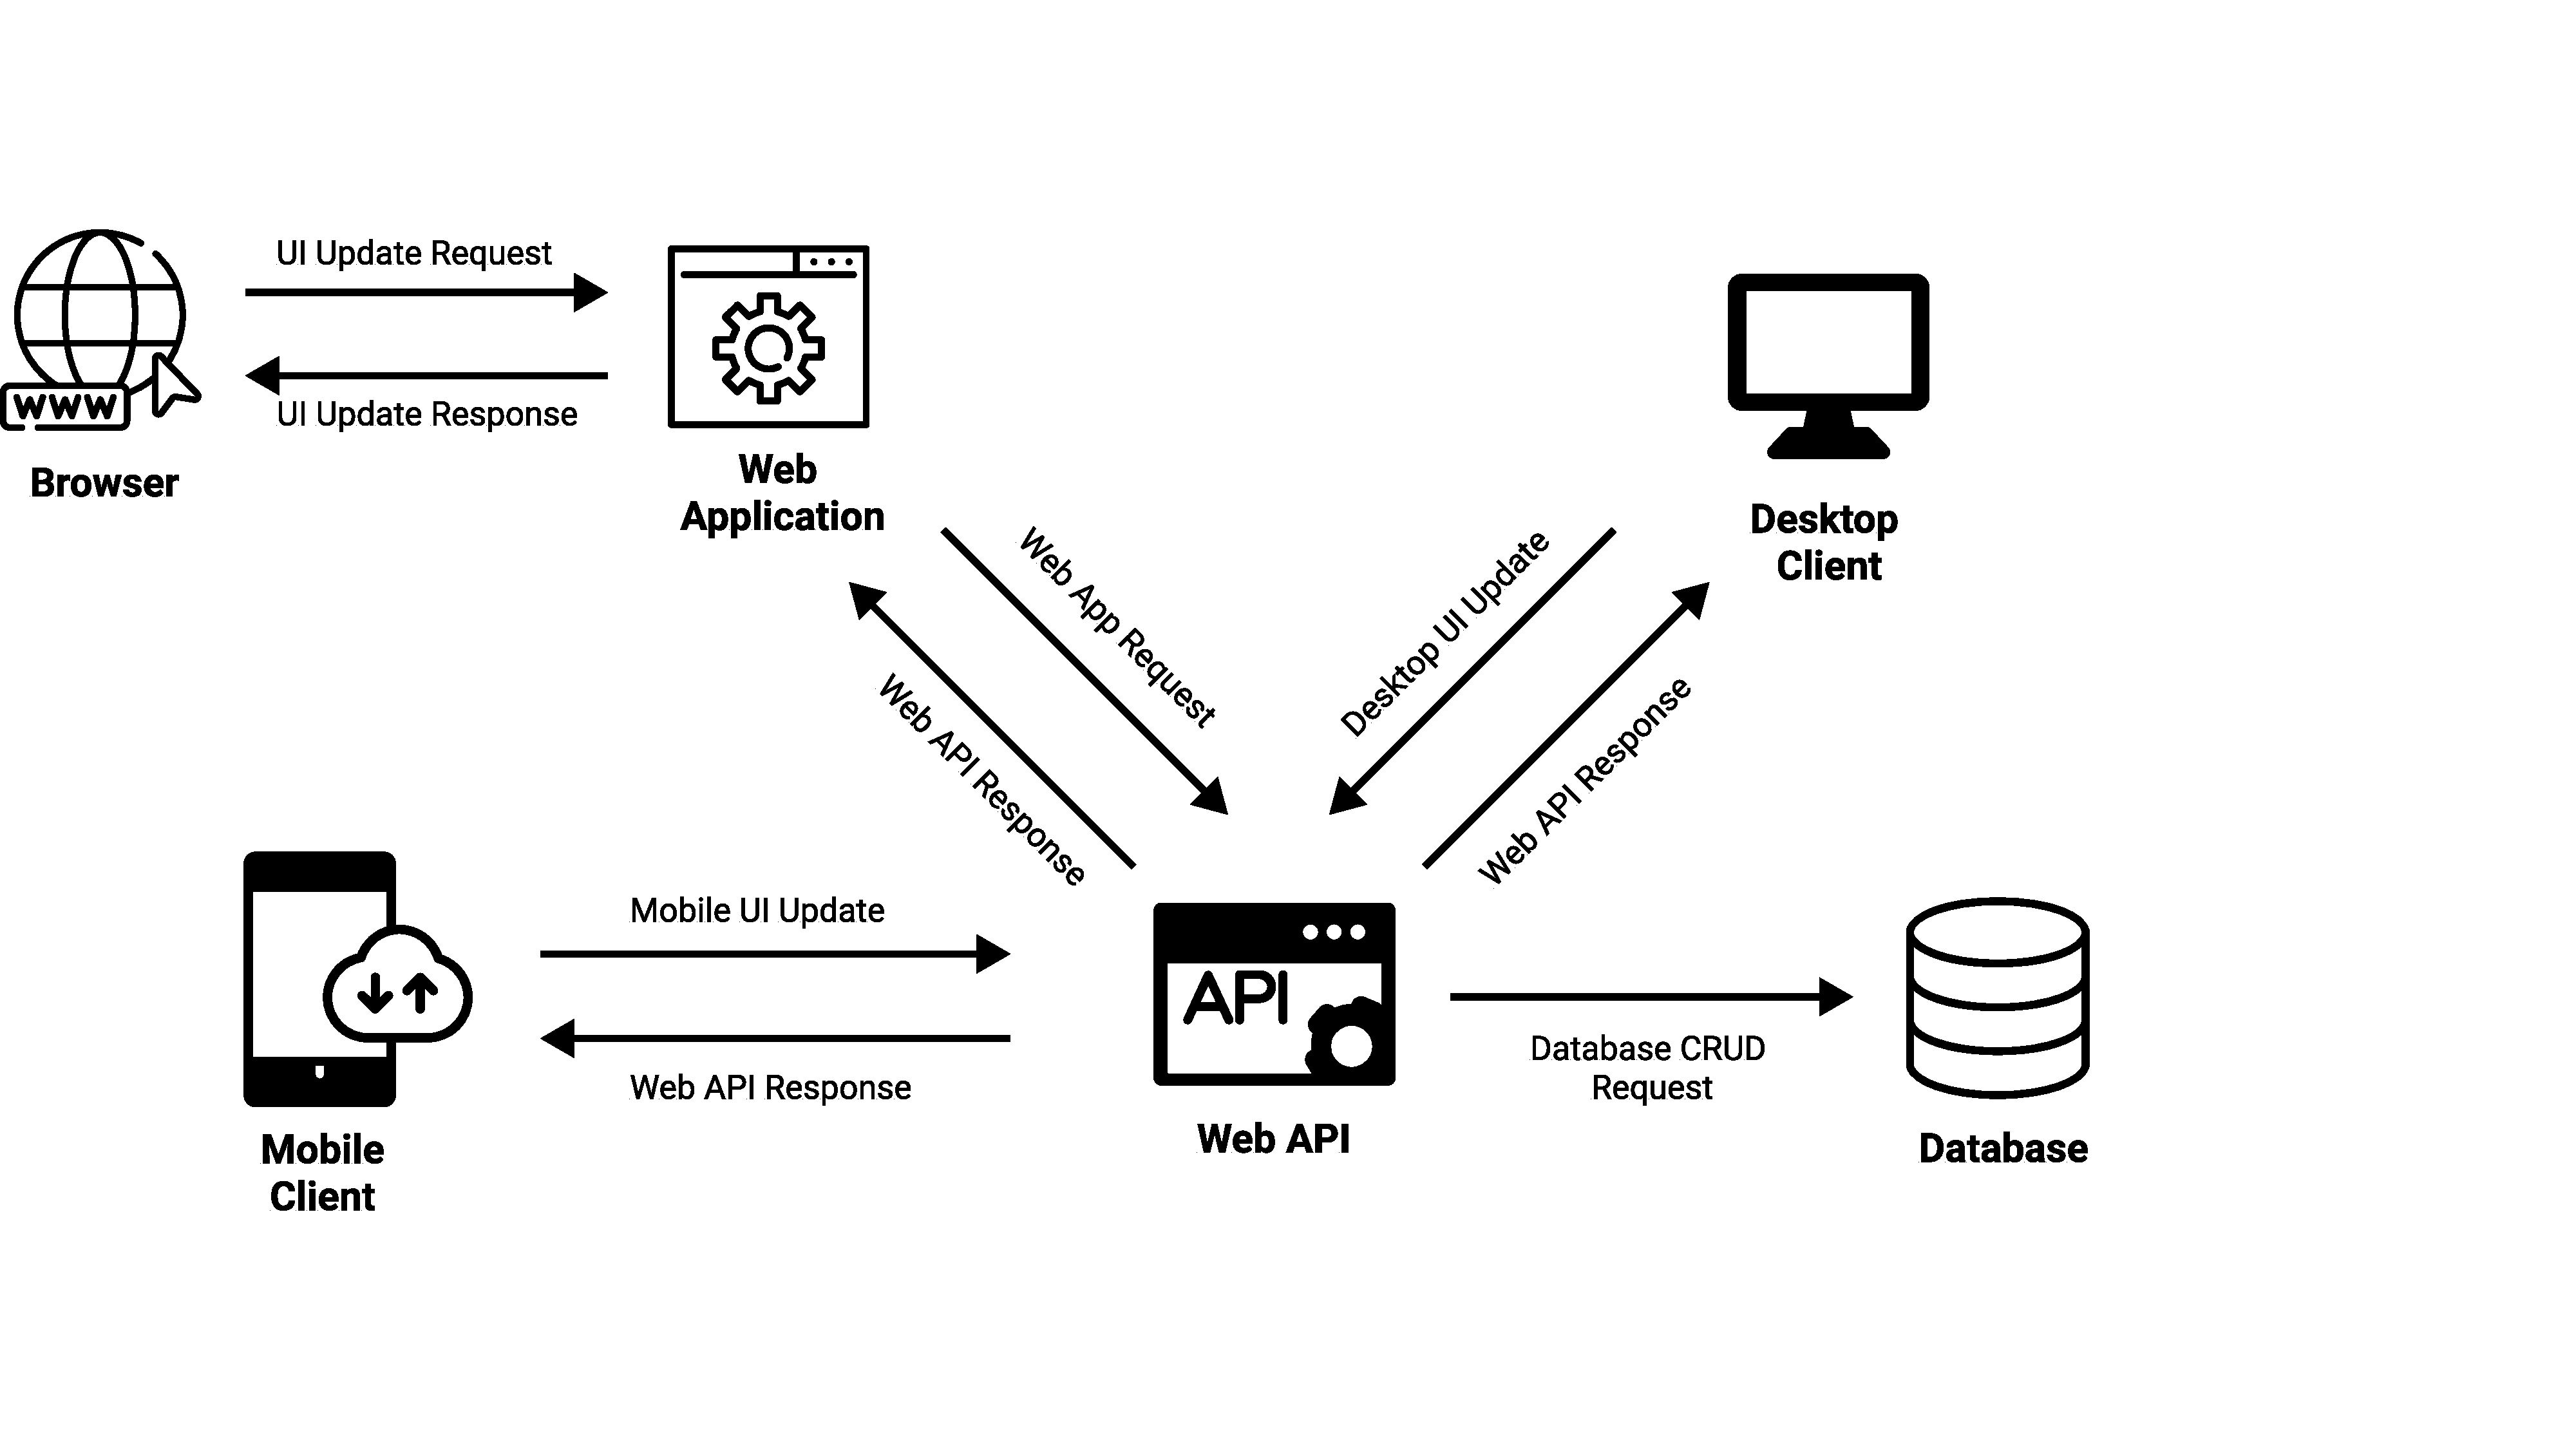
\includegraphics[width=1.2\textwidth]{Pictures/Threat_Modeling}
    \caption{Database diagram.}\label{fig:figure6}
\end{figure}

\begin{enumerate}
    \item \textbf{Browser UI Update Request}
    \begin{itemize}
        \item \textbf{Treat 1.1.} An adversary can perform action on behalf of other user due to lack of controls against cross domain requests.
        \item \textbf{Treat 1.2.} An adversary may bypass critical steps or perform actions on behalf of other users (victims) due to improper validation logic.
        \item \textbf{Treat 1.3.} An adversary can reverse weakly encrypted or hashed content.
        \item \textbf{Treat 1.4.} An adversary may gain access to sensitive data from log files.
        \item \textbf{Treat 1.5.} An adversary can spoof the target web application due to insecure TLS certificate configuration.
        \item \textbf{Treat 1.6.} An adversary can steal sensitive data like user credentials.
        \item \textbf{Treat 1.7.} An adversary can gain access to sensitive data stored in Web App's config files.
        \item \textbf{Treat 1.8.} An adversary can gain access to sensitive data by performing SQL injection through Web App.
        \item \textbf{Treat 1.9.} An attacker steals messages off the network and replays them in order to steal a user's session.
        \item \textbf{Treat 1.10.} An adversary can deface the target web application by injecting malicious code or uploading dangerous files.
        \item \textbf{Treat 1.11.} An adversary may spoof Desktop Web Browser (Chrome) and gain access to Web Application.
        \item \textbf{Treat 1.12.} An adversary can create a fake website and launch phishing attacks.
        \item \textbf{Treat 1.13.} Attackers can steal user session cookies due to insecure cookie attributes.
        \item \textbf{Treat 1.14.} An adversary can get access to a user's session due to insecure coding practices.
        \item \textbf{Treat 1.15.} An adversary can get access to a user's session due to improper logout and timeout.
        \item \textbf{Treat 1.16.} Attacker can deny the malicious act and remove the attack foot prints leading to repudiation issues.
        \item \textbf{Treat 1.17.} An adversary may gain access to sensitive data from uncleared browser cache.
        \item \textbf{Treat 1.18.} An adversary can gain access to sensitive information through error messages.
        \item \textbf{Treat 1.19.} An adversary can gain access to sensitive data by sniffing traffic to Web Application.
        \item \textbf{Treat 1.20.} An adversary can gain access to certain pages or the site as a whole.
        \item \textbf{Treat 1.21.} An adversary may gain access to unmasked sensitive data such as credit card numbers.
    \end{itemize}
    \item \textbf{Web App Request}
    \begin{itemize}
        \item \textbf{Treat 2.1.} An adversary may gain unauthorized access to Web API due to poor access control checks.
        \item \textbf{Treat 2.2.} An adversary can gain access to sensitive information from an API through error messages.
        \item \textbf{Treat 2.3.} An adversary can gain access to sensitive data by sniffing traffic to Web API\@.
        \item \textbf{Treat 2.4.} An adversary can gain access to sensitive data stored in Web API's config files.
        \item \textbf{Treat 2.5.} Attacker can deny a malicious act on an API leading to repudiation issues.
        \item \textbf{Treat 2.6.} An adversary may spoof Mango Web Application and gain access to Web API\@.
        \item \textbf{Treat 2.7.} An adversary may inject malicious inputs into an API and affect downstream processes.
        \item \textbf{Treat 2.8.} An adversary can gain access to sensitive data by performing SQL injection through Web API\@.
    \end{itemize}
    \item \textbf{Web API Response}
    \begin{itemize}
        \item \textbf{Treat 3.1.} An adversary can reverse weakly encrypted or hashed content.
        \item \textbf{Treat 3.2.} An adversary may gain access to sensitive data from log files.
        \item \textbf{Treat 3.3.} An adversary can gain access to sensitive information through error messages.
        \item \textbf{Treat 3.4.} Attacker can deny the malicious act and remove the attack foot prints leading to repudiation issues.
        \item \textbf{Treat 3.5.} An adversary can spoof the target web application due to insecure TLS certificate configuration.
        \item \textbf{Treat 3.6.} An adversary can steal sensitive data like user credentials.
        \item \textbf{Treat 3.7.} An adversary can create a fake website and launch phishing attacks.
    \end{itemize}
    \item \textbf{CRUD Request}
    \begin{itemize}
        \item \textbf{Treat 4.1.} An adversary can gain unauthorized access to database due to loose authorization rules.
        \item \textbf{Treat 4.2.} An adversary can gain access to sensitive PII or HBI data in database.
        \item \textbf{Treat 4.3.} An adversary can gain access to sensitive data by performing SQL injection.
        \item \textbf{Treat 4.4.} An adversary can deny actions on database due to lack of auditing.
        \item \textbf{Treat 4.5.} An adversary can tamper critical database securables and deny the action.
        \item \textbf{Treat 4.6.} An adversary may leverage the lack of monitoring systems and trigger anomalous traffic to database.
        \item \textbf{Treat 4.7.} An adversary can gain unauthorized access to database due to lack of network access protection.
    \end{itemize}
    \item \textbf{Mobile UI Update}
    \begin{itemize}
        \item \textbf{Treat 5.1.} An adversary can gain access to sensitive data by performing SQL injection through Web API.
        \item \textbf{Treat 5.2.} An adversary can reverse engineer and tamper binaries.
        \item \textbf{Treat 5.3.} An adversary may inject malicious inputs into an API and affect downstream processes.
        \item \textbf{Treat 5.4.} An adversary may spoof Mobile App (IOS, Android) and gain access to Web API\@.
        \item \textbf{Treat 5.5.} An adversary obtains refresh or access tokens from Mobile App (IOS, Android) and uses them to
        obtain access to the Mango Web API\@.
        \item \textbf{Treat 5.6.} Attacker can deny a malicious act on an API leading to repudiation issues.
        \item \textbf{Treat 5.7.} An adversary can gain access to sensitive data stored in Web API's config files.
        \item \textbf{Treat 5.8.} An adversary can gain sensitive data from mobile device.
        \item \textbf{Treat 5.9.} An adversary can gain access to sensitive data by sniffing traffic to Web API\@.
        \item \textbf{Treat 5.10.} An adversary can gain access to sensitive data by sniffing traffic from Mobile client.
        \item \textbf{Treat 5.11.} An adversary can gain access to sensitive information from an API through error messages.
        \item \textbf{Treat 5.12.} An adversary may gain unauthorized access to Web API due to poor access control checks.
        \item \textbf{Treat 5.13.} An adversary may jail break into a mobile device and gain elevated privilege.
    \end{itemize}
\end{enumerate}

\subsection{System Requirements}\label{subsec:system-requirements}
Prior to software module implementation, it is essentially important to define the functionality module will obtain.
In this section we discuss functional and non-functional requirements of secure instant messaging system from customer's prospective.
Generally, there are three forms of software product requirements: business, functional, and non-functional.
Business requirements [\cite{dilworth2007creation}] typically answer how the product will address the needs of your company and its users.
They also reveal the business model of the app and what problems it can solve.
Functional requirements [\cite{malan2001functional}] are about functionalities that will be implemented in the application.
Non-functional requirements [\cite{chung2012non}] describe how these functionalities will be implemented.

To compete with successful and commonly used instant messaging platforms, your service has to offer great functionality.
So first, let’s define the core features of a messaging app.
\begin{itemize}
    \item Registration
    \item Authentication
    \item Authorization
    \item Adding contacts
    \item Sending messages and media to individuals
    \item Creating groups
    \item Sending messages and media to groups user stories
    \item Viewing message history
    \item Profile settings
\end{itemize}
Note that Authentication [\cite{burrows1989logic}] means confirming your own identity,
whereas Authorization [\cite{fagin1978authorization}] means being allowed access to the particular part of the system.

\subsection{Registration user stories}\label{subsec:registration}
\begin{itemize}
    \item As an unregistered user, I want to tap “register” so that I can see the registration form.
    \item As an unregistered user, I want to use my phone number to register so that my account is tied to my phone number.
    \item As an unregistered user, I want to use my e-mail to register so that my account is tied to my phone number.
    \item As an unregistered user, I want to add a display name during registration so that other users can find
    my account not only by my phone number or e-mail.
    \item As an unregistered user, I want to choose how to receive the registration confirmation via SMS or e-mail
    so that notification is sent by SMS or e-email.
    \item As an unregistered user, I want to receive the registration confirmation via SMS or Email so that
    I can activate my account.
\end{itemize}

\subsection{Authentication user stories}\label{subsec:authentication-user-stories}
\begin{itemize}
    \item As an un-authenticated user, I want to authenticate myself using both combinations email-password
    and phone-password so that I use the specified form with two inputs.
    \item As an authenticated user, I want my session on each device to least 7 days
    so that after 7 days of inactivity device will be logged out automatically.
\end{itemize}

\subsection{Adding contacts user stories}\label{subsec:adding-contacts}
\begin{itemize}
    \item As an authorized user, I want to add other user to my contact list so that each user profile has a dedicated button.
    \item As an authorized user, I want to remove the user from my contact list so that each contact profile has a dedicated button.
    \item As an authorized user, I want to send message to the user from my contact list so that each contact profile has a dedicated button.
\end{itemize}

\subsection{Sending messages and media to individuals user stories}
\label{subsec:sending-messages-and-media-feature-user-stories}
\begin{itemize}
    \item As an authorized user, I want to send a text message so that another user sees my message.
    \item As an authorized user, I want to send a document so that another user sees the document I sent.
    \item As an authorized user, I want to tap "Edit" on my message, so that I edit the message sent by myself.
    \item As an authorized user, I want to tap "Delete" on my message, so that I delete the message sent by myself.
\end{itemize}

\subsection{Creating groups user stories}\label{subsec:creating-groups-feature-user-stories}
\begin{itemize}
    \item As a registered user, I want to tap "details" -> "create group" in sidebar so that create a new group.
    \item As a registered user, I want to tap "details" -> "new chat" in sidebar, so that create a new direct chat with specified user.
    \item As a registered user, I want to join public groups, so that there is a button "join" on chat layout.
    \item As a registered user, I want to start secret chats with users from my contact list so that we can send messages that stay only on our devices.
    \item As a registered user, I want my secret chats to be device-specific so that I can see a secret chat only on the device that I used to start this chat.
    \item As a member of a secret chat, I want my secret messages to be protected from forwarding so that secret messages stay in secret chats.
    \item As a member of a secret chat, I want to get a notification when another member of the secret chat takes a screenshot of it.
\end{itemize}

\subsection{Sending messages and media to groups user stories}
\label{subsec:sending-messages-and-media-to-groups}
\begin{itemize}
    \item As an authorized user, I want to send a text message so that all members of a group see my message.
    \item As an authorized user, I want to send a document so that all members of a group see the document I sent.
    \item As an authorized user, I want to tap "Edit" on my message, so that I edit the message sent by myself.
    \item As an authorized user, I want to tap "Delete" on my message, so that I delete the message sent by myself.
\end{itemize}

\subsection{Viewing message history user stories}\label{subsec:viewing-message-history-feature-user-stories}
\begin{itemize}
    \item As an authorized user, I want to be able to view a message history of particular chat or group
    so that I see a list of my active chats on the UI\@.
\end{itemize}

\subsection{Profile settings user stories}\label{subsec:profile-settings-user-stories}
\begin{itemize}
    \item As an authorized user, I want to be able to change my personal information so that I use a specified form.
    \item As an authorized user, I want reset password, so that my password will change.
    \item As an authorized user, I want to tap "Logout" button so that current device will be logged out from the system.
    \item As an authorized user, I want to tap "Logout all" button, so that all my authorized devices will be
    logged out from the system.
\end{itemize}


\subsection{Web service architecture}\label{subsec:web-service-architecture}
\textbf{Motivation.} Implementing the instant messenger system, we consider applying a well-known N-tier
Monolithic Architecture [\cite{bucchiarone2018monolithic}], which provides a time-proven model that allows software
developers to create flexible and reusable applications.

However, during the implementation of monolith it is very important to avoid the cases of crucial over-engineering
of the system that leads to useless complication of the code base.
For the developers, it is a vital point to follow the KISS [\cite{alwin2016kiss}] and YAGNI [\cite{da2018evolution}]
software development principles in order not to reach
\href{https://github.com/smartstore/SmartStoreNET/blob/4.x/src/Presentation/SmartStore.Web/Controllers/CatalogHelper.cs}
{thousands lines}
of code in a single class.

One would suggest to use nowadays popular Microservices Architecture, thinking about scalability [\cite{brataas2004exploring}],
an ability of the system to handle large numbers of users distributed over geographically large areas without
notably affecting the overall performance of the system.
However, the effect of Microservices is being felt only for quite large and complex systems,
not the case of our yet simple application.
According to \href{https://martinfowler.com/bliki/MonolithFirst.html}{Martin Fowler},
\begin{quote}
    \textit{you shouldn't start a new project with microservices, even if you're sure your application will be big enough to
    make it worthwhile.}
\end{quote}
which is so-called \textit{Monolith first} approach.
Makes sense to begin an implementation from \textit{Modular monolith}, a monolith with minimized coupling between the
software components, where splitting to microservice won't be a time and financial expensive operation.
Following plot demonstrates the relation between the complexity and profits between monolith and microservices

\begin{figure}[H]
    \centering
    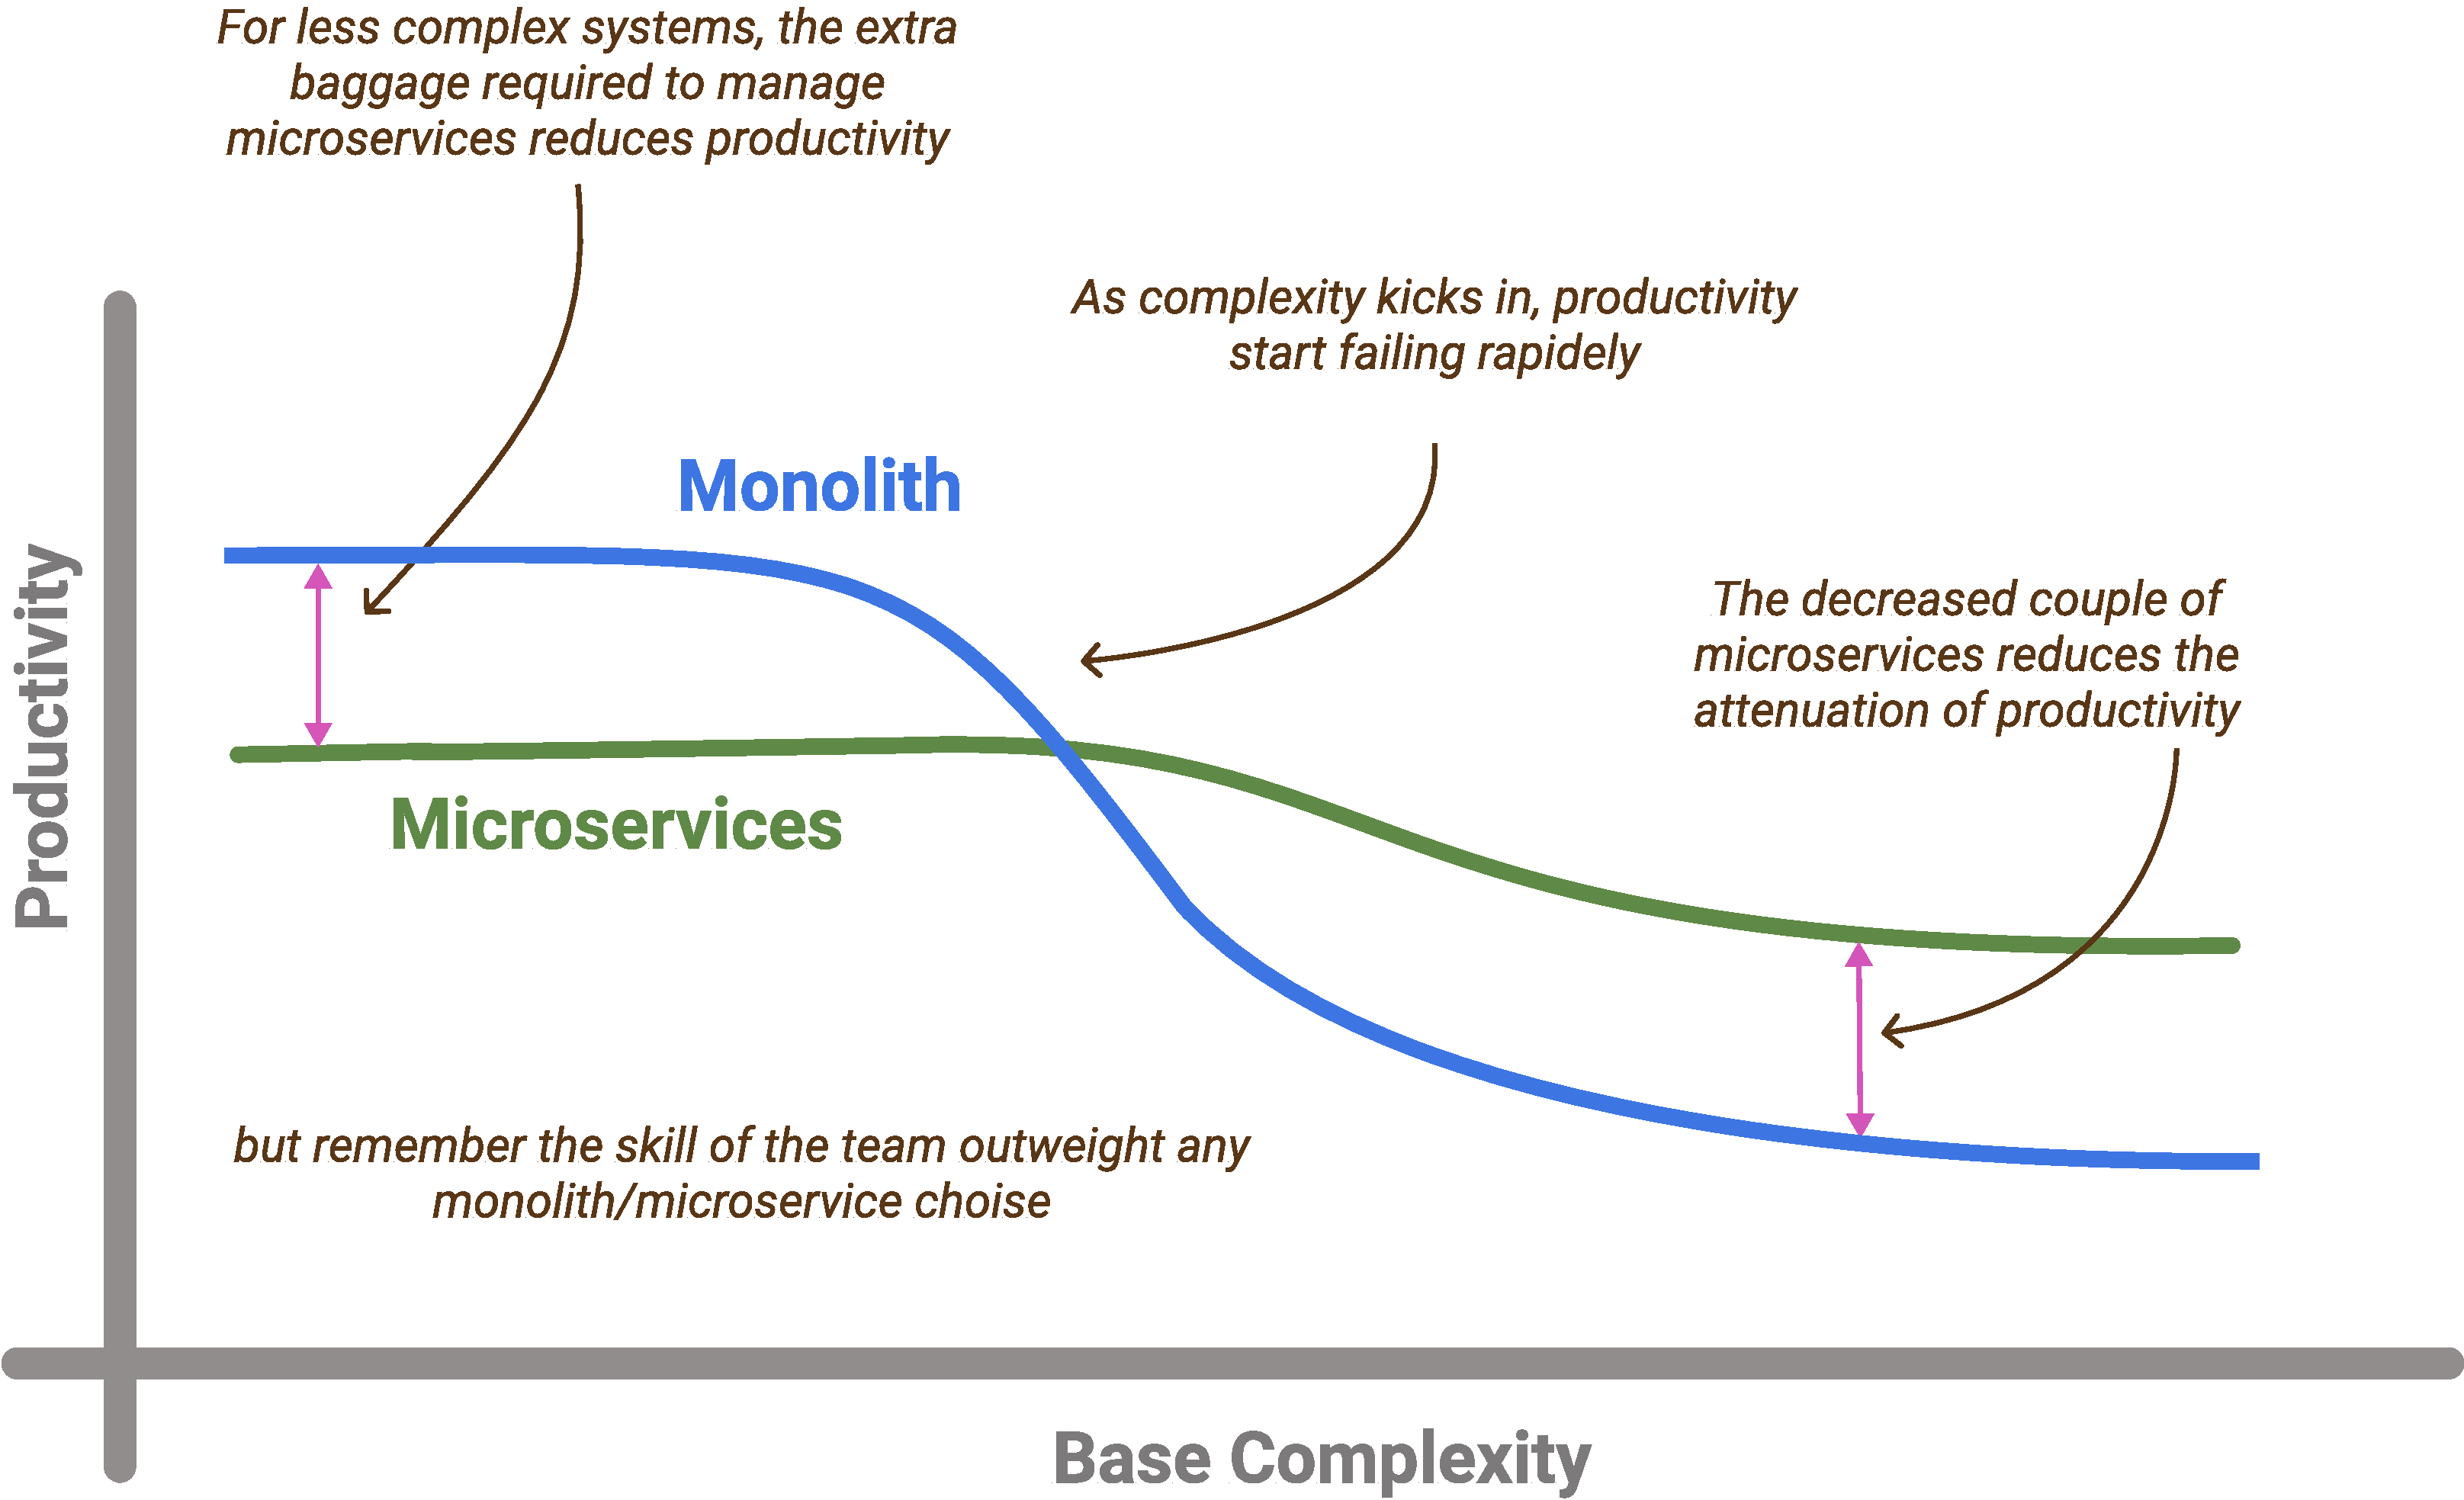
\includegraphics[width=1\textwidth]{Pictures/02_Monolith_and_Microservices_complexity}
    \caption{Relation between system complexity and architectures.
    Source: \href{https://martinfowler.com/bliki/MicroservicePremium.html}{Martin Fowler.}}
    \label{fig:monolith_vs_microservice}
\end{figure}

A layered architecture usually consists of Presentation layer, Business logic layer, Data access layer.
By segregating the project into layers, developers reach the options to modify or add a specific layer
without reworking the entire application.

\begin{itemize}
    \item \textit{Presentation Layer.} Graphic user interface or API gateway.
    \item \textit{Application Logic.} Encapsulates the means of interaction with user.
    For example, push-notifications e-mail notification, sms notifications etc.
    \item \textit{Business Logic.} Encapsulates the logic of clint's request handling.
    For example, service layer.
    \item \textit{Data Access Layer.} Responsible for logging, database access and other services required to support
    Business Logic layer.
\end{itemize}

\begin{figure}[H]
    \centering
    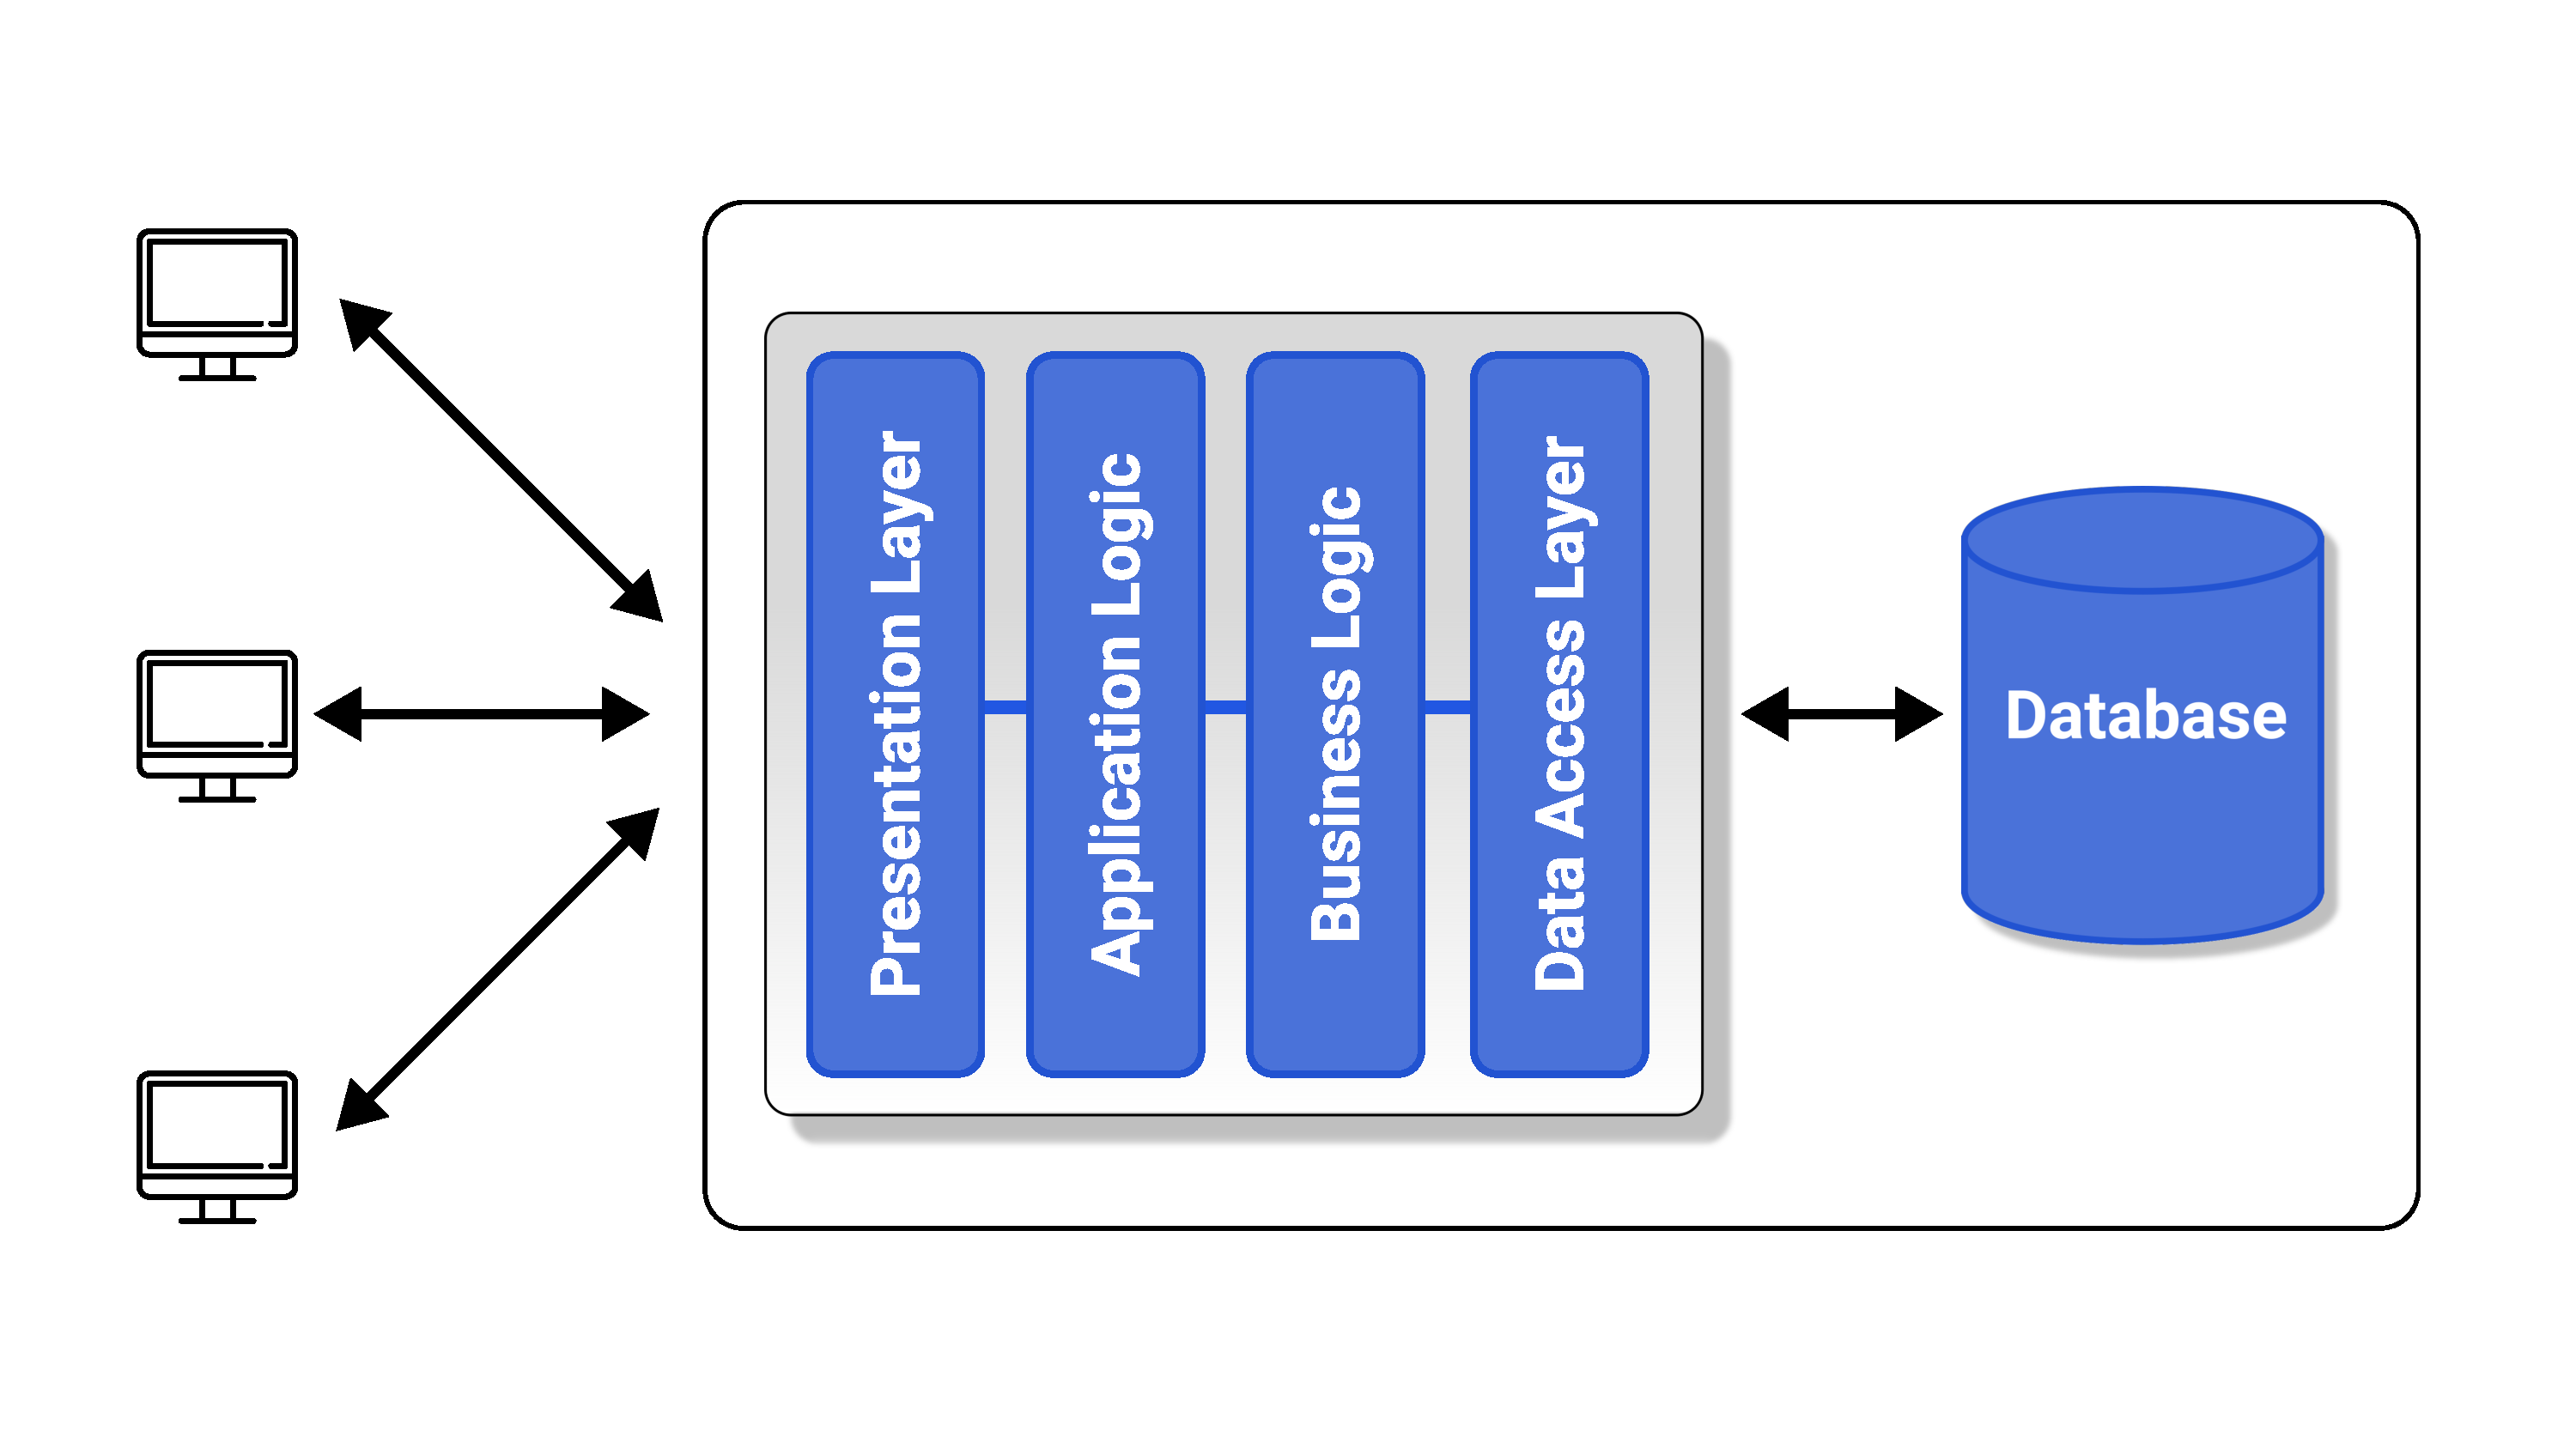
\includegraphics[width=1\textwidth]{Pictures/03_Monolith_concept_diagram}
    \caption{Monolith concept diagram.}\label{fig:figure2}
\end{figure}

\textbf{Monolithic Architecture: Cons and Props.} A monolith is built as a large system with a single code base and
deployed as a single unit, usually behind a load balancer.
Monoliths offer several advantages, particularly when it comes to operational overhead requirements.
Here are some of those basic benefits:

\begin{itemize}
    \item \textit{Simplicity.} Monolithic architectures are simple to build and deploy.
    These applications can scale horizontally, by running several copies of the application behind a load balancer.
    With a single codebase, monolithic apps can easily handle cross-cutting concerns, such as logging,
    configuration management and performance monitoring.
    Another advantage associated with the simplicity of monolithic applications is easier deployment.
    When it comes to monolithic applications, you do not have to handle many deployments but just one.
    \item \textit{Performance.} Components in a monolith typically share memory which is faster than service-to-service
    communications using IPC [\cite{proctor1999linux}] or other mechanisms.
    \item \textit{Easier debugging and testing.}
    In contrast to the microservices, monolithic applications are much easier to debug and test.
    Since that monolithic application is a single indivisible unit the process of end-to-end testing is much faster.
    \item \textit{Easier development.} As long as the monolithic approach is a standard way of building applications,
    any engineering team has the right knowledge and capabilities to develop a monolithic application.
\end{itemize}

However, the drawback of monolithic architectures hides in their tight coupling.
Over time, monolithic components and layers become tightly coupled and entangled, effecting management, scalability
and continuous deployment.
Another disadvantages of the monoliths include:
\begin{itemize}
    \item \textit{Understanding.} When a monolithic application's code base grows up, it becomes too complicated to understand.
    Obviously, huge code base of monolithic app is hard to manage therefore.
    \item \textit{Reliability.} Entire application down may be caused by an error in every single component.
    \item \textit{Updates.} Single and large code base causes the needs to redeploy an application on every single update.
    \item \textit{Technology stack.} Technology stack of the monolithic app is limited by the technologies and providers
    used from the beginning of development.
    It makes technology stack changes to be expensive in terms of finances and time.
    \item \textit{Scalability.} Application's components cannot be scaled independently, an entire application should be scaled.
\end{itemize}

\textbf{Minimization of services coupling.} As we see, the monolith has its own disadvantages, like for instance:
understanding the project structure, reliability concerns, technology stack limitations, scalability limitations.
Obviously, some of these disadvantages cannot be mitigated because of the nature of the monolith.
However, the complexity and coupling problem can be minimized applying certain approaches.
Frequent violation of the single-responsibility principle of SOLID during implementing service components
in business logics layer causes the over-complication of codebase over the time.
The reason is that service components keep the huge number of methods in order to handle all possible CRUD requests
to the database without any bounded context.
Although, the SOLID rules are very powerful in solving designated code issues, it is necessary to apply them very carefully,
since that most of them require high level of abstractions, which increases in size the code base and complicates the
solution.
Do not overcomplicate the solution without any reason following \textit{Open-Closed Principle}.
Schematically, the service entity is as follows
\begin{figure}[H]
    \centering
    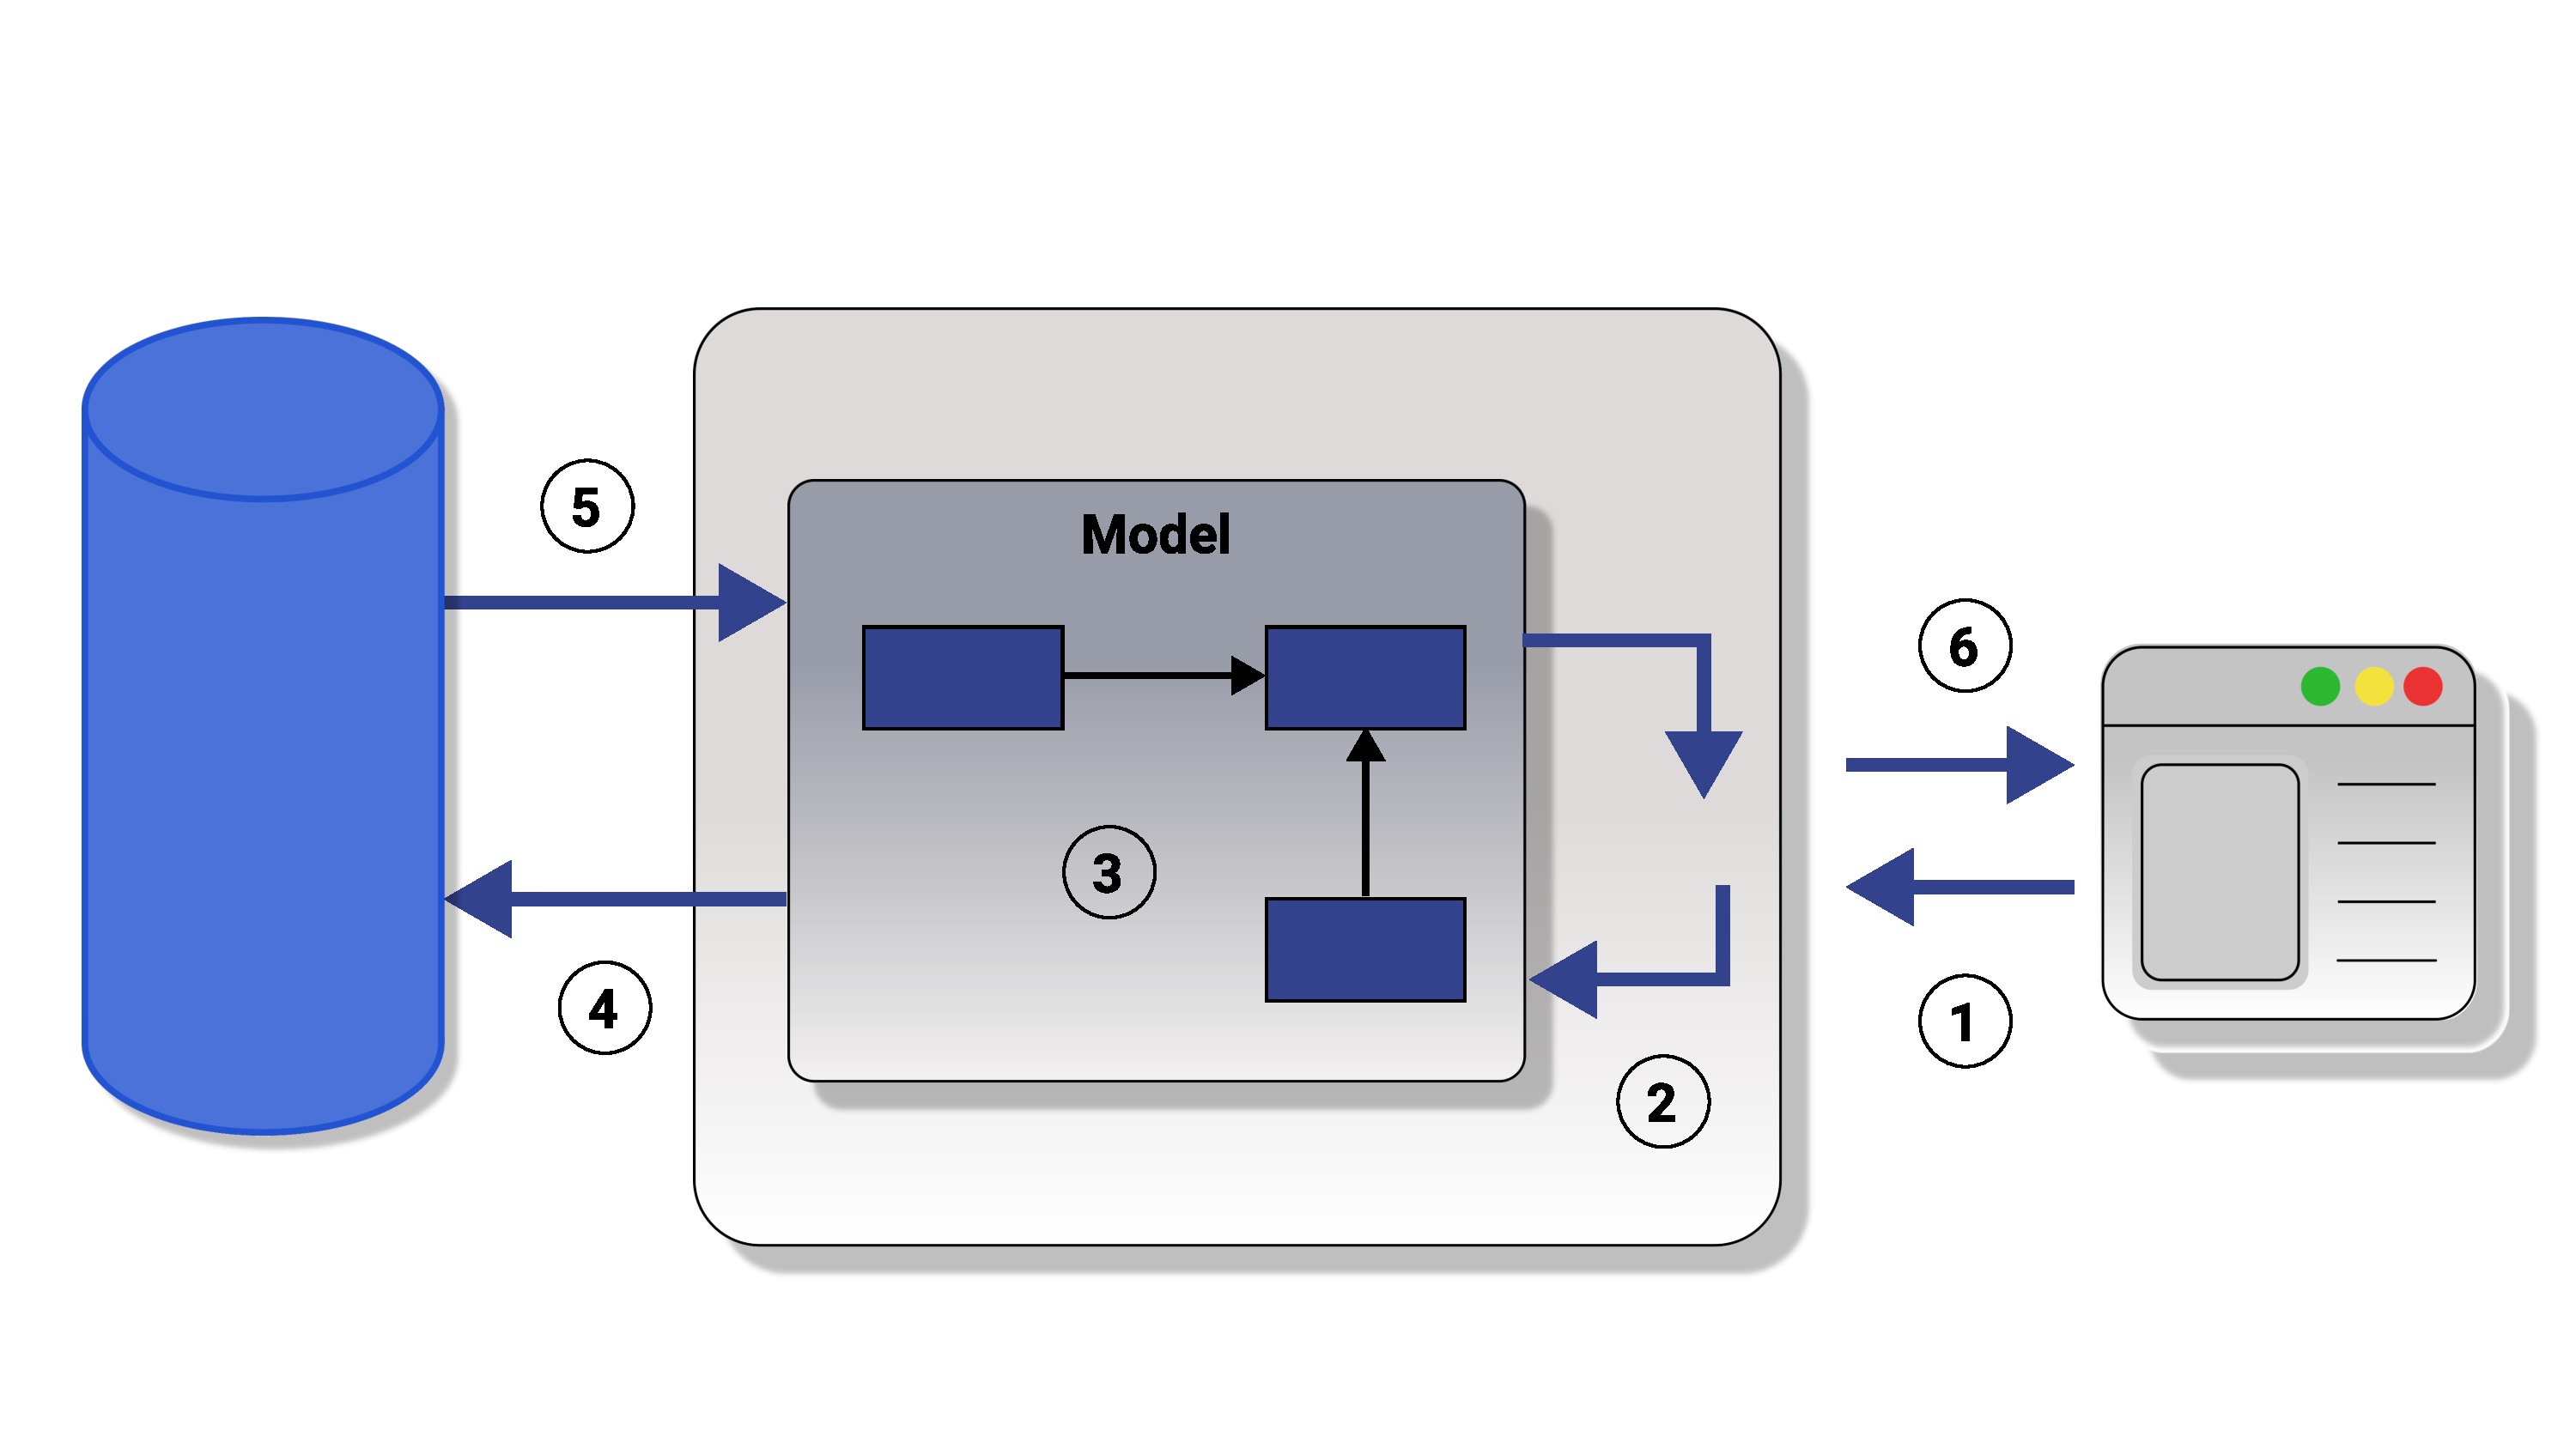
\includegraphics[width=1\textwidth]{Pictures/04_Service_entity_concept_diagram}
    \caption{Service entity concept diagram.
    Source: \href{https://martinfowler.com/bliki/CQRS.html}{Martin Fowler}.}\label{fig:figure9}
\end{figure}
Where the steps are
\begin{enumerate}
    \item User makes a change in UI\@.
    \item Change forwarded to model.
    \item Model executes validation and business logic.
    \item Model updates the database.
    \item Model reads from database.
    \item Service updates presentation from query model.
\end{enumerate}

To minimize the natural disadvantages of the monolithic architecture like complexity and high tight coupling of the components
we have to recall the design patterns [\cite{rising1998design}].
In particular, the mediator pattern helps to decouple the components.
Mediator -- is a behavioral design pattern [\cite{rasche2016building}] that allows the communication between two entities,
such that entities doesn't know each other.
Therefore, the program components depend only on a single mediator instance instead of being coupled to multiple of their
colleagues.
In context of .NET platform there are many implementations of the Mediator, the most widely known and used is the
\href{https://github.com/jbogard/MediatR}{MediatR}, which we use in our project.

Another mindset we are going to use in order to minimize complexity and coupling of monolith is Command-Query
Responsibility Segregation (CQRS) principle.
In brief, it stands that read (query) and write (command) requests should be segregated by their responsibilities.
Using CQRS and Mediator together greatly simplifies the project structure and minimizes coupling between business
logic layer components.
CQRS is a pattern that first described by Greg Young [\cite{young2010cqrs}] and its conceptual diagram as follows

\begin{figure}[H]
    \centering
    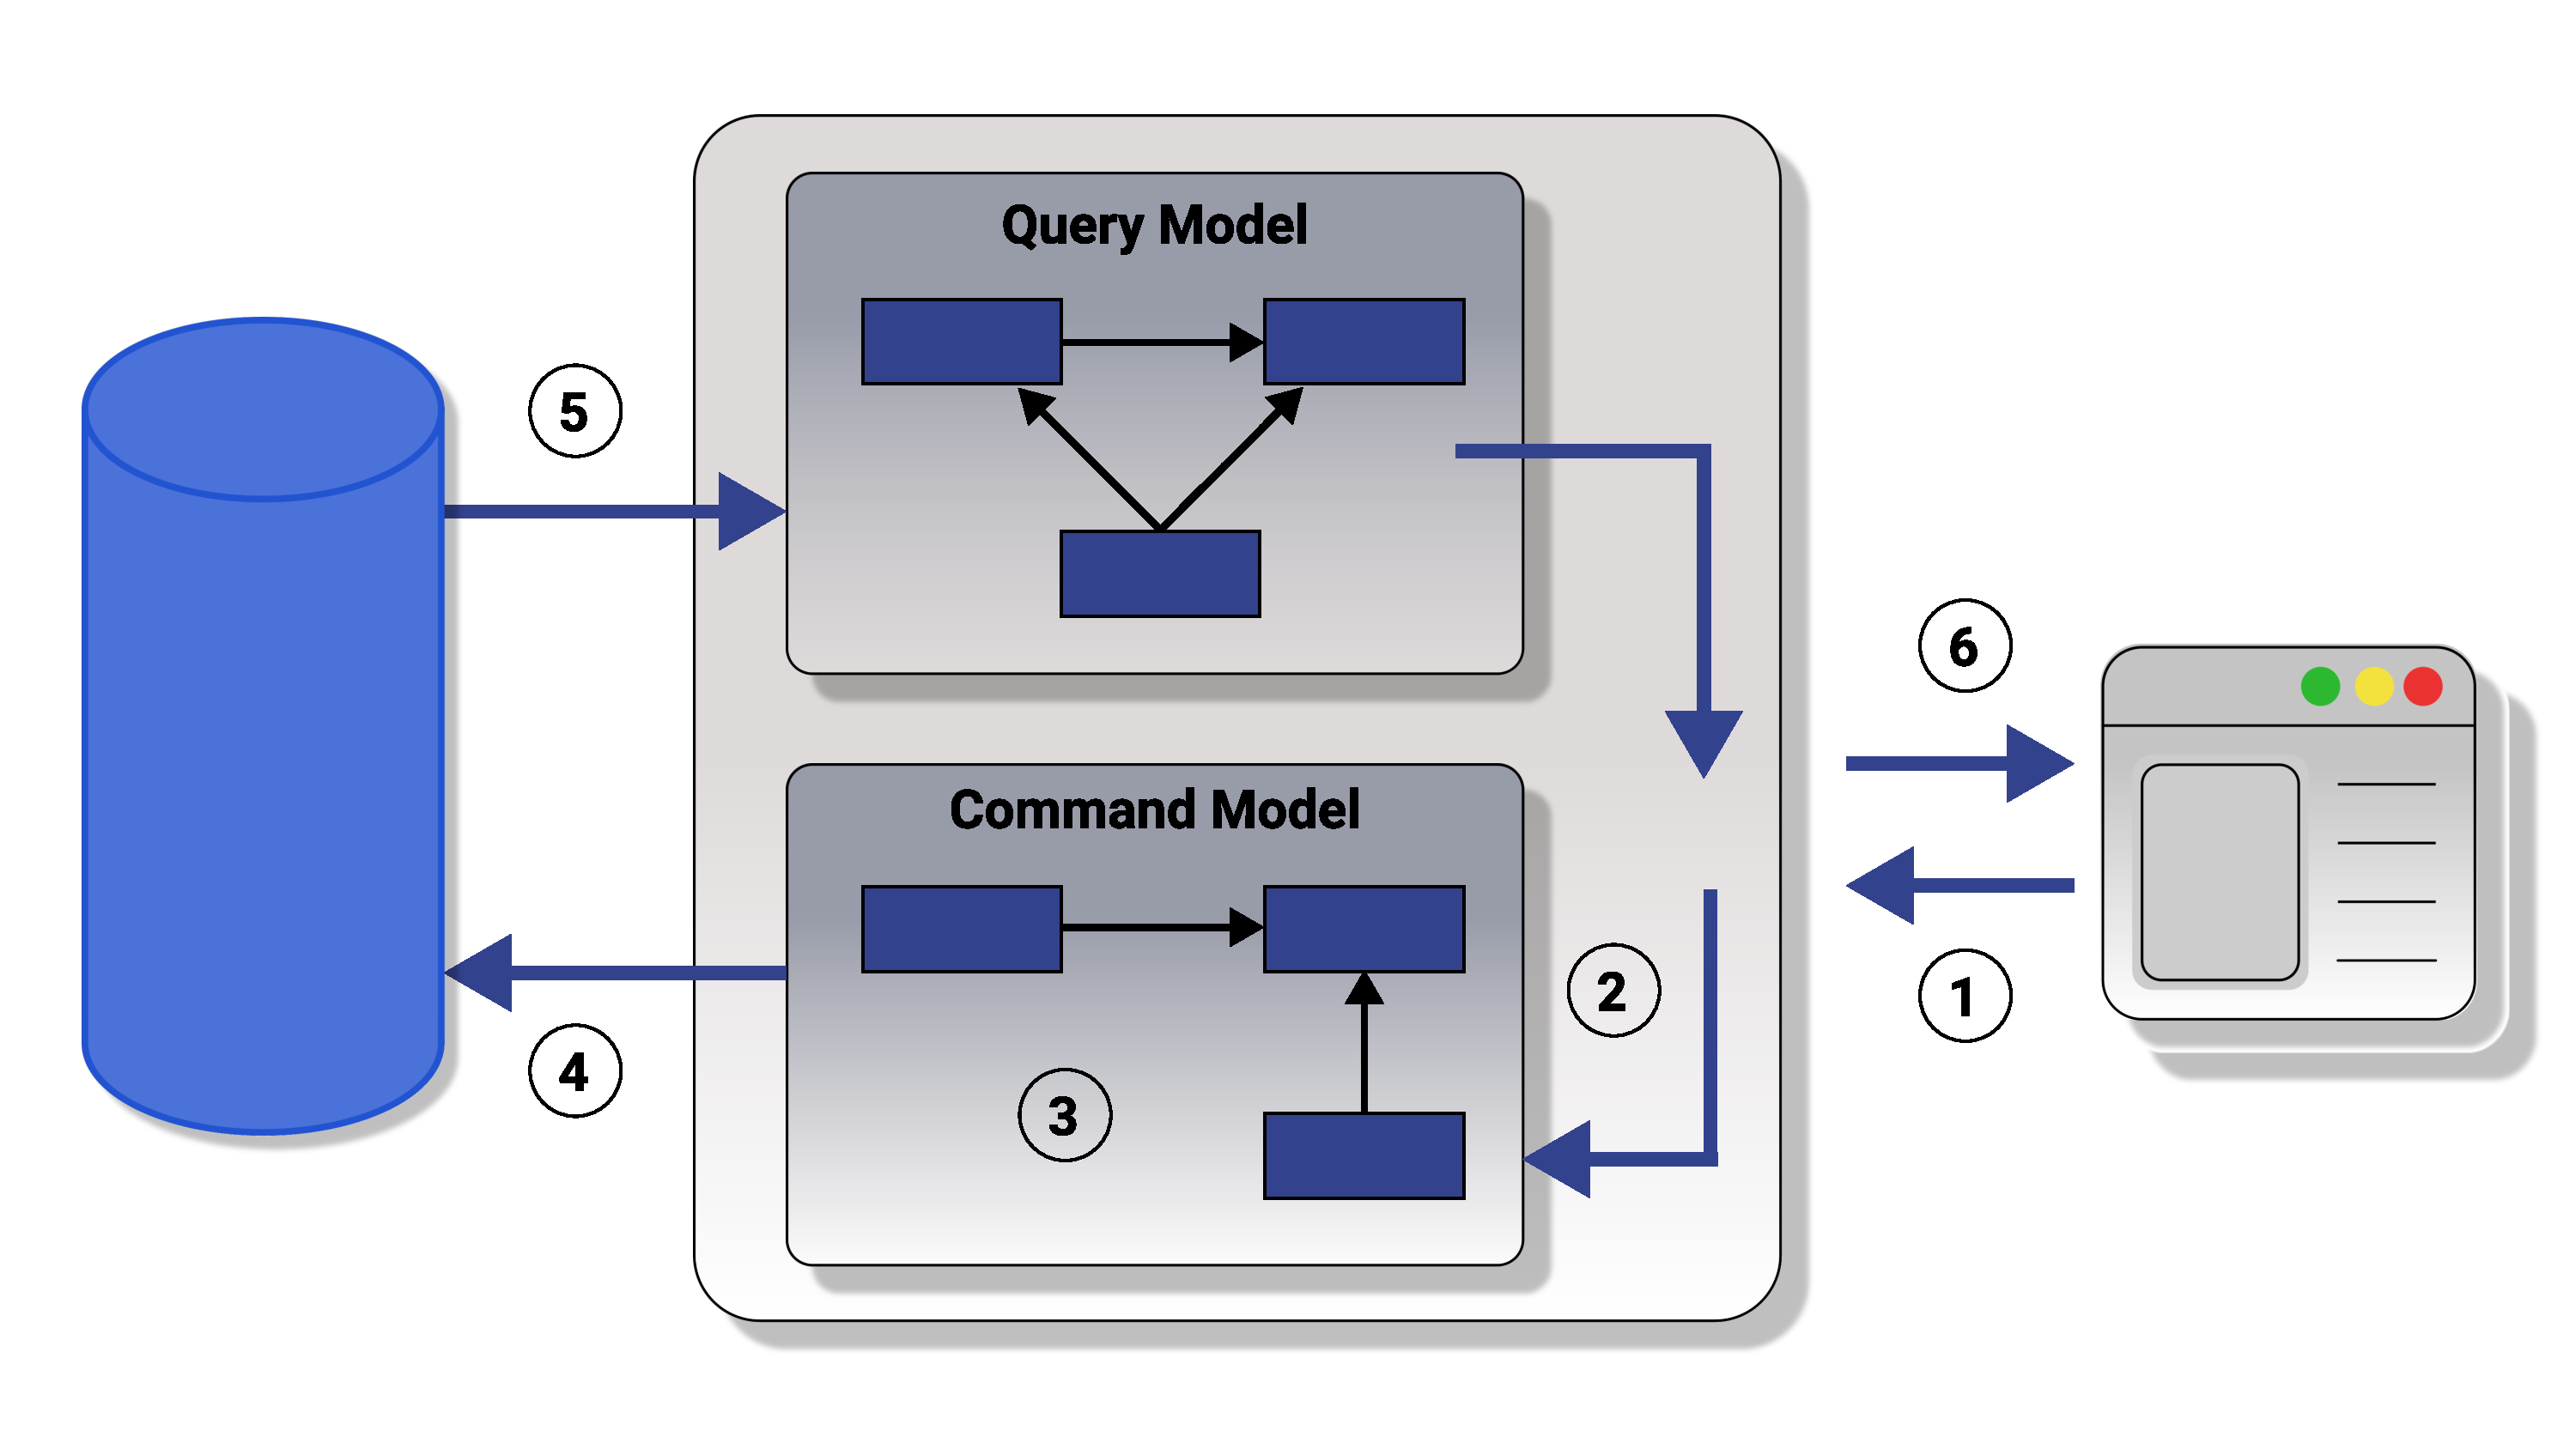
\includegraphics[width=1\textwidth]{Pictures/05_CQRS_concept_diagram}
    \caption{CQRS concept diagram.
    Source: \href{https://martinfowler.com/bliki/CQRS.html}{Martin Fowler}.}
    \label{fig:figure}
\end{figure}

\begin{enumerate}
    \item User makes a change in UI\@.
    \item Application routes information to command model.
    \item Command model executes validation and business logic.
    \item Command model updates the database.
    \item Query model reads from database.
    \item Query service update presentation from query model.
\end{enumerate}

\subsection{Authorization mechanism}\label{subsec:authorization-mechanism}
\textbf{Motivation.} In this section we describe the processes of Authentication and Authorization in the system.
It is worth to remember the meaning of Authentication and Authorization definitions.
Authentication -- is the process of ascertaining that somebody really is who they claim to be [\cite{burrows1989logic}].
Authorization refers to rules that determine who is allowed to do what [\cite{fagin1978authorization}].
For example, Adam may be authorized to create and delete databases, while Catherine is only authorized to read.
The two concepts are completely orthogonal and independent, but both are central to security design, and the
failure to get either one correct opens up the avenue to compromise.
In terms of web apps, very crudely speaking, authentication is when you check login credentials to see if you recognize
a user as logged in, and authorization is when you look up in your access control whether you allow the user to view,
edit, delete or create content.
Currently, there are two widely-known authentication methods, that are cookie authentication and JWT authentication.

\textbf{JWT Tokens.}
JSON Web Token or JWT is an open standard [\cite{jones2015rfc}] that defines a compact and self-contained way for securely
exchanging information between parties as a Javascript Object Notation (JSON) object [\cite{jones2015json}].
This information can be verified and trusted thanks to digital signature of the sender.
JSON Web Tokens could be signed using a secret with the HMAC,
stands for Hash-based Message Authentication Code algorithm [\cite{wang2004hmac}] or a public-private key pair using
the Rivest, Shamir and Adleman algorithm [RSA~\cite{wiener1990cryptanalysis}] or Elliptic Curve Digital Signature Algorithm
[ECDSA~\cite{johnson2001elliptic}].
Here are some scenarios JSON Web Tokens are useful in:

\begin{itemize}
    \item \textit{Authorization.} Is the most widely known scenario for using JWT\@.
    Once the user logs in, each further request will include the JWT to request header, allowing the user to access routes,
    services, and resources that are permitted with that token.
    Single Sign On is a feature that widely uses JWT nowadays, because of its small overhead and its ability to be easily
    used across different domains.
    Thanks to JWTs we are able to use Single Sign On feature, because of the JWTs' small overhead and ability to be
    used across different domains avoiding CORS errors.
    \item \textit{Information Exchange.} JSON Web Tokens may be used as secure way of communication.
    Because JWTs can be signed, it is simple to verify and identify the sender.
    Moreover, since that signature is calculated combining the header and the payload of the token, it is possible to verify
    that token has not been changed on the road.
\end{itemize}
JSON Web Token consists of the three parts separated by dots: Header, Payload, Signature.
Therefore, a JWT typically looks like
\begin{center}
    \begin{spverbatim}
        eyJhbGciOiJIUzI1NiIsInR5cCI6IkpXVCJ9.
        eyJqdGkiOiJmZDNjNjdjNS1jNmZmLTRhNWQtY
        TE2Ni05OGVjZTFiNzc1MmIiLCJyb2xlIjoiVX
        NlciIsIm5iZiI6MTYzMTU1MjQ5NiwiZXhwIjo
        xNjMxNTUyNzk2LCJpYXQiOjE2MzE1NTI0OTYs
        ImlzcyI6Imh0dHBzOi8vbWFuZ28tbWVzc2VuZ
        2VyLWFwcC5oZXJva3VhcHAuY29tIiwiYXVkIj
        oiaHR0cHM6Ly9tYW5nby1tZXNzZW5nZXItYXB
        wLmhlcm9rdWFwcC5jb20vYXBpIn0.
        locHt8ow1lFnGGZ_aFFvXI09dD4y1r594XQF2
        -6YxCw
    \end{spverbatim}
\end{center}
Let's discuss each part separately.
\begin{itemize}
    \item \textit{Header.} Typically, consists of two parts: the type of the token, and the signing algorithm
    being used, like \texttt{HMAC SHA256} or \texttt{RSA}.
    Example of header is as follows

    \begin{spverbatim}
    {
        "alg": "HS256",
        "typ": "JWT"
    }
    \end{spverbatim}

    After that, JSON is Base64 [\cite{josefsson2003rfc3548}] encoded to create the header part of the JWT\@.
    \item \textit{Payload.} The second part of the token is the payload with the entity claims.
    Claims are statements about the user and additional data.
    Claims are of the following types: registered, public and private claims.
    \begin{itemize}
        \item Registered claims.
        A set of predefined claims.
        Registered claims are not mandatory but recommended, to provide a set of useful and interoperable claims.
        For example, the following are registered claims
        \texttt{iss} stands for issuer,
        \texttt{exp} stands for expiration time,
        \texttt{sub} stands for subject,
        \texttt{aud} stands for audience,
        and \href{https://tools.ietf.org/html/rfc7519#section-4.1}{others}.
        The claim names are only three characters long to maintain the compactness of the JWT\@.
        \item Public claims.
        These claims can be defined freely.
        In order to avoid collisions public claims should be defined in the
        \href{https://www.iana.org/assignments/jwt/jwt.xhtml}{IANA JSON Web Token Registry}
        or to be defined in a form of URI which contains a collision resistant namespace.
        \item Private claims. These claims are the claims which can be created manually in order to share
        the information between the parties.
    \end{itemize}
    An example payload could be:

    \begin{spverbatim}
    {
        "sub": "10203040",
        "name": "Alice Fox",
        "approved": true
    }
    \end{spverbatim}

    The payload is then Base64 encoded to form the second part of the JSON Web Token.
    It is recommended to put secret information in payload or header only in encrypted form, since that Base64 is encoding
    only and can be read by anyone.
    \item \textit{Signature.} The signature part of the JWT is created combining the Base64 encoded
    header and payload using the specified in header algorithm.
    For instance, if the HMAC SHA256 algorithm is used, the signature will be created in the following way:

    \begin{spverbatim}
        HMACSHA256(
        base64UrlEncode(header) + "." +
        base64UrlEncode(payload),
        secret)
    \end{spverbatim}

    The signature is used to ensure that tokens wasn't changed during the exchange between parties,
    so-called Man in the middle attack.
    \item \textit{Conclusions.} JWT is three Base64 encoded strings separated by dots that can be
    used in authorization and information exchange over HTTP,
    JWTs are more compact related to XML-based standards like SAML\@.
\end{itemize}

As to the projects concerns, we should handle multiple client applications, e.g desktop,
web, mobile etc, therefore JWT authorization fits perfectly.

\textbf{JWT Authorization.} In authentication, when the user successfully logs in using their credentials,
a JSON Web Token will be returned.
Since tokens are credentials, great care must be taken to prevent security issues.
In general, you should not keep tokens longer than required.
You also should not store sensitive session data in browser storage due to lack of security.
Whenever the user wants to access a protected route or resource, the user agent should send the JWT,
typically in the Authorization header using the Bearer schema.
The content of the header should look like the following:
\begin{spverbatim}

    Authorization: Bearer <token>

\end{spverbatim}
This can be, in certain cases, a stateless authorization mechanism.
The server's protected routes will check for a valid JWT in the Authorization header, and if it's present,
the user will be allowed to access protected resources.
If the JWT contains the necessary data, the need to query the database for certain operations may be reduced,
though this may not always be the case.
If the token is sent in the Authorization header, Cross-Origin Resource Sharing (CORS) won't be an issue
as it doesn't use cookies.
Generally, the workflow is as follows
\begin{enumerate}
    \item User provides credentials in order to authenticate to the system.
    \item Server verifies user's authentication, fetches the login and password in database.
    \item If authentication is successful, server creates session then writes this session to the database.
    \item Server generates a pair of access JWT token and refresh token as GUID.
    \item Server sends to client access token and refresh token.
    \item Client saves the pair of access and refresh tokens.
    \item User requests resource using received token passed to the request header.
    \item The server check user's claims and proceeds or declines request.
\end{enumerate}

The eighth point is the authorization.
As a result, token stored on the client and used when it is necessary to authorize the requests.
When a hacker tries to replace the data in the header or payload the token will become invalid,
therefore the signature will not match the original values.
So, the hacker hasn't any possibility to generate a new signature since that encryption secret key stored on the server.
Access token in form of JWT is used for request authorization and for storing the additional information
about user like identifier, display name and others.
Refresh token in form of GUID issued by server based on successful authentication results and used
to get new access-refresh token pair.
Also, it is worth to add a few basic rules about JWT secure usage.
The lifetime of JWT should not be long since that stolen JWT cannot be revoked.
Randall Degges advices to follow the regulations [\cite{RDegges}]
\begin{itemize}
    \item JWT should have a short lifetime, since it cannot be revoked.
    \item JWT should be used in a single time, e.g.\ JWT per request.
\end{itemize}
However, extremely short lifetimes of the tokens would affect the overall performance of the system.
Therefore, we consider access token's lifetime to be 5 minutes and refresh token's 7 days.

For each request client preliminarily checks access token's lifetime.
If access token it expired, client sends request for updating a pair of access-refresh tokens.
For more confidence, we can update tokens a few seconds earlier.
That is, the case when the API receives an expired access token is practically excluded.
However, we are able to consider the case of interception of the request on \texttt{401UNAUTHORIZED} http status code.
The following diagram demonstrates the process of requesting the resource

\begin{figure}[H]
    \centering
    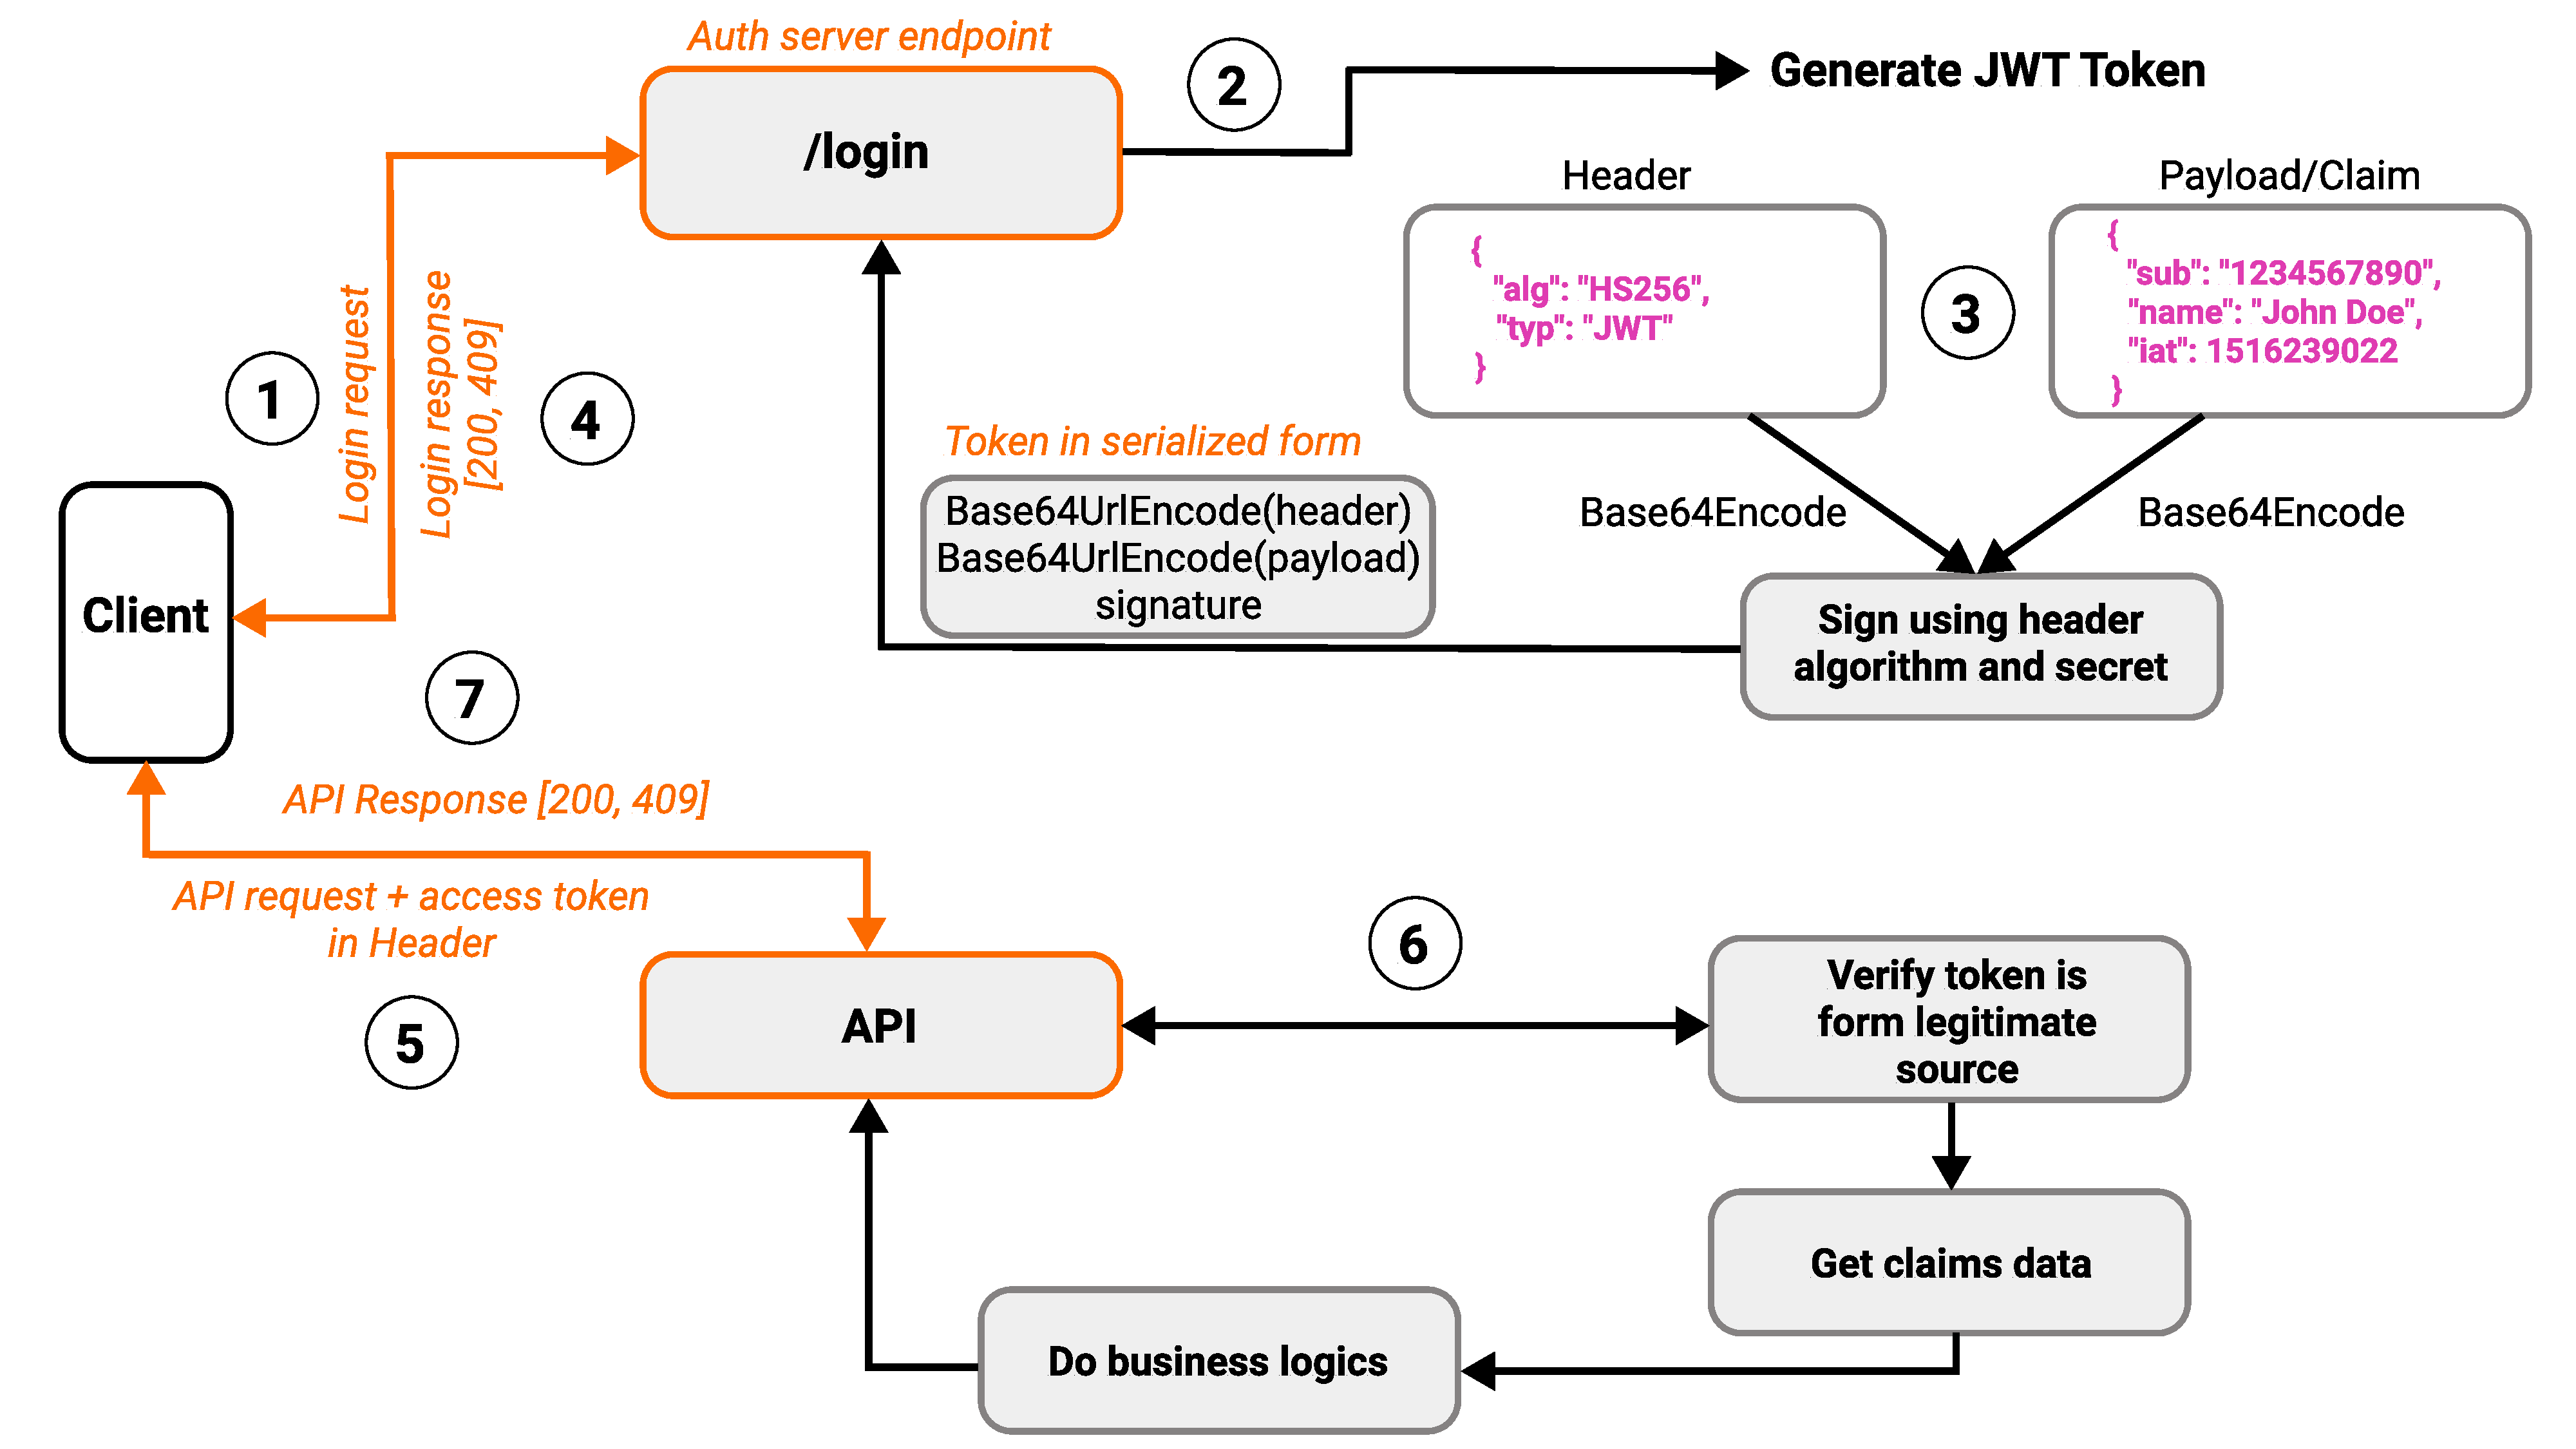
\includegraphics[width=1\textwidth]{Pictures/06_JWT_authorization_concept_diagram}
    \caption{JWT Authorization concept diagram.}\label{fig:figure3}
\end{figure}

By steps, the process is
\begin{itemize}
    \item \textbf{Step 1.} \textit{Client} application sends authentication request to
    the \textit{Auth server endpoint} provided user credentials in request body.
    \item \textbf{Step 2.} \textit{Auth server endpoint} responses to the \textit{Client} with the following
    HTTP response codes:
    \begin{itemize}
        \item \texttt{409CONFLICT}: Invalid credentials.
        \item \texttt{200SUCCESS}: Returns a pair of access and refresh tokens.
        \begin{itemize}
            \item \textbf{Step 3.} \textit{Auth server} generates a pair of access and refresh tokens
            \begin{itemize}
                \item \textit{Auth server} fetches user data and claims.
                \item \textit{Auth server} creates new session instance in database.
                \item \textit{Auth server} Base64 encodes access token's Header.
                \item \textit{Auth server} Base64 encodes access token's Payload.
                \item \textit{Auth server} generates access token's Signature using encoded token's
                Header and Payload signed by means of the \texttt{HMACSHA256} algorithm and secret.
            \end{itemize}
        \end{itemize}
    \end{itemize}
    \item \textbf{Step 4.} JWT access token in serialized form and refresh token in form of GUID are
    returned in response with \texttt{200SUCCESS} http status code to the \textit{Client} from the \textit{Auth server}.
    \item \textbf{Step 5.} \textit{Client} queries the \textit{API} providing access token as
    Bearer in request header.
    \item \textbf{Step 6.} \textit{API} validates the token claims in order to authorize user
    \begin{itemize}
        \item If authorized: \textit{API} handles the request, goes to \textbf{Step 7}.
        \item Otherwise: returns error with \texttt{401UNAUTHORIZED} http status code.
    \end{itemize}
    \item \textbf{Step 7.} \textit{} returns response with \texttt{200SUCCESS} or \texttt{409CONFLICT}
    http status codes to the client, according to business logic layer implementation.
\end{itemize}

\subsection{Diffie-Hellman key exchange}\label{subsec:diffie-hellman-key-exchange}
\textbf{Motivation.} End-to-end encryption is an encryption such that the only communicating parties
are able to decrypt the data.
It means that even system administrators are not able to decrypt the messages transmitted between parties
via their communication channel.
End-to-end encryption can be reached via numerous approaches.
Generally, there are two ways to implement E2E encryption
\begin{itemize}
    \item Sharing public key to be used in encryption of the secret message, then encryption is done by the
    public key's owner, so-called asymmetric encryption.
    For example, RSA algorithm.
    \item Asymmetric key exchange, where parties firstly exchanging the keys, then symmetrically encrypting
    the transferred data.
    For instance, Diffie--Hellman key exchange and AES256 encryption using common secret.
\end{itemize}
The most important aspect here is to securely store the secrets on the user's client application.
Due to storage issues, it doesn't make sense to implement E2E encryption for web
and desktop clients, like it is done in nowadays popular Telegram Messenger
[\cite{job2015modified,suvsanka2017security,lee2017security}].
Telegram uses the huge and heavy \texttt{MTProto 2.0} cryptographic protocol, based on DH key exchange and further AES256
symmetric encryption.
According to the project concerns, the E2E encryption via Diffie--Hellman key exchange and AES256
to be considered and implemented, the next section is about.

\textbf{Diffie–-Hellman key exchange.} Diffie--Hellman (DH) protocol is a method of asymmetric exchange
of the cryptographic keys for a group of two or more participants,
developed in 1976 by cryptographers Ralph Merkle, Whitfield Diffie and Martin Hellman.
In contrast to symmetric key exchange, the Diffie–-Hellman protocol eliminates the direct transfer of the shared secret
between the participants, each participant computes a shared secret with its own private-public key pair.
The Diffie–-Hellman protocol is based on a one-way function of the form

\begin{equation}
    A = G ^ a \bmod P \label{eq:equation}
\end{equation}

where $A$ is the user's public key,
$a$ is the user's private key,
$P=2Q+1$ is modulus, such that 2048 bits safe-prime because $Q$ is also prime,
$G$ is generator such that $G$ is primitive root modulo $P$.
We say that $G$ is primitive root modulo $P$ if for each $1 \leq a \leq P - 1$ the $A = G ^ a \bmod P$
is unique and belong to the set $\{1, 2, \dots, P-1\}$.
The period of such cyclic group $\mathbb{Z}_{P}$ is $P-1$ then.

Thus, the safety of the Diffie--Hellman protocol is based on the discrete logarithm problem, which is unsolvable
in polynomial time if the constants $G$ and $P$ are chosen correctly.
Graphically, the flow of the Diffie--Hellman protocol can be expressed through the
analogy with mixing paints, as below picture shows
\begin{figure}[H]
    \centering
    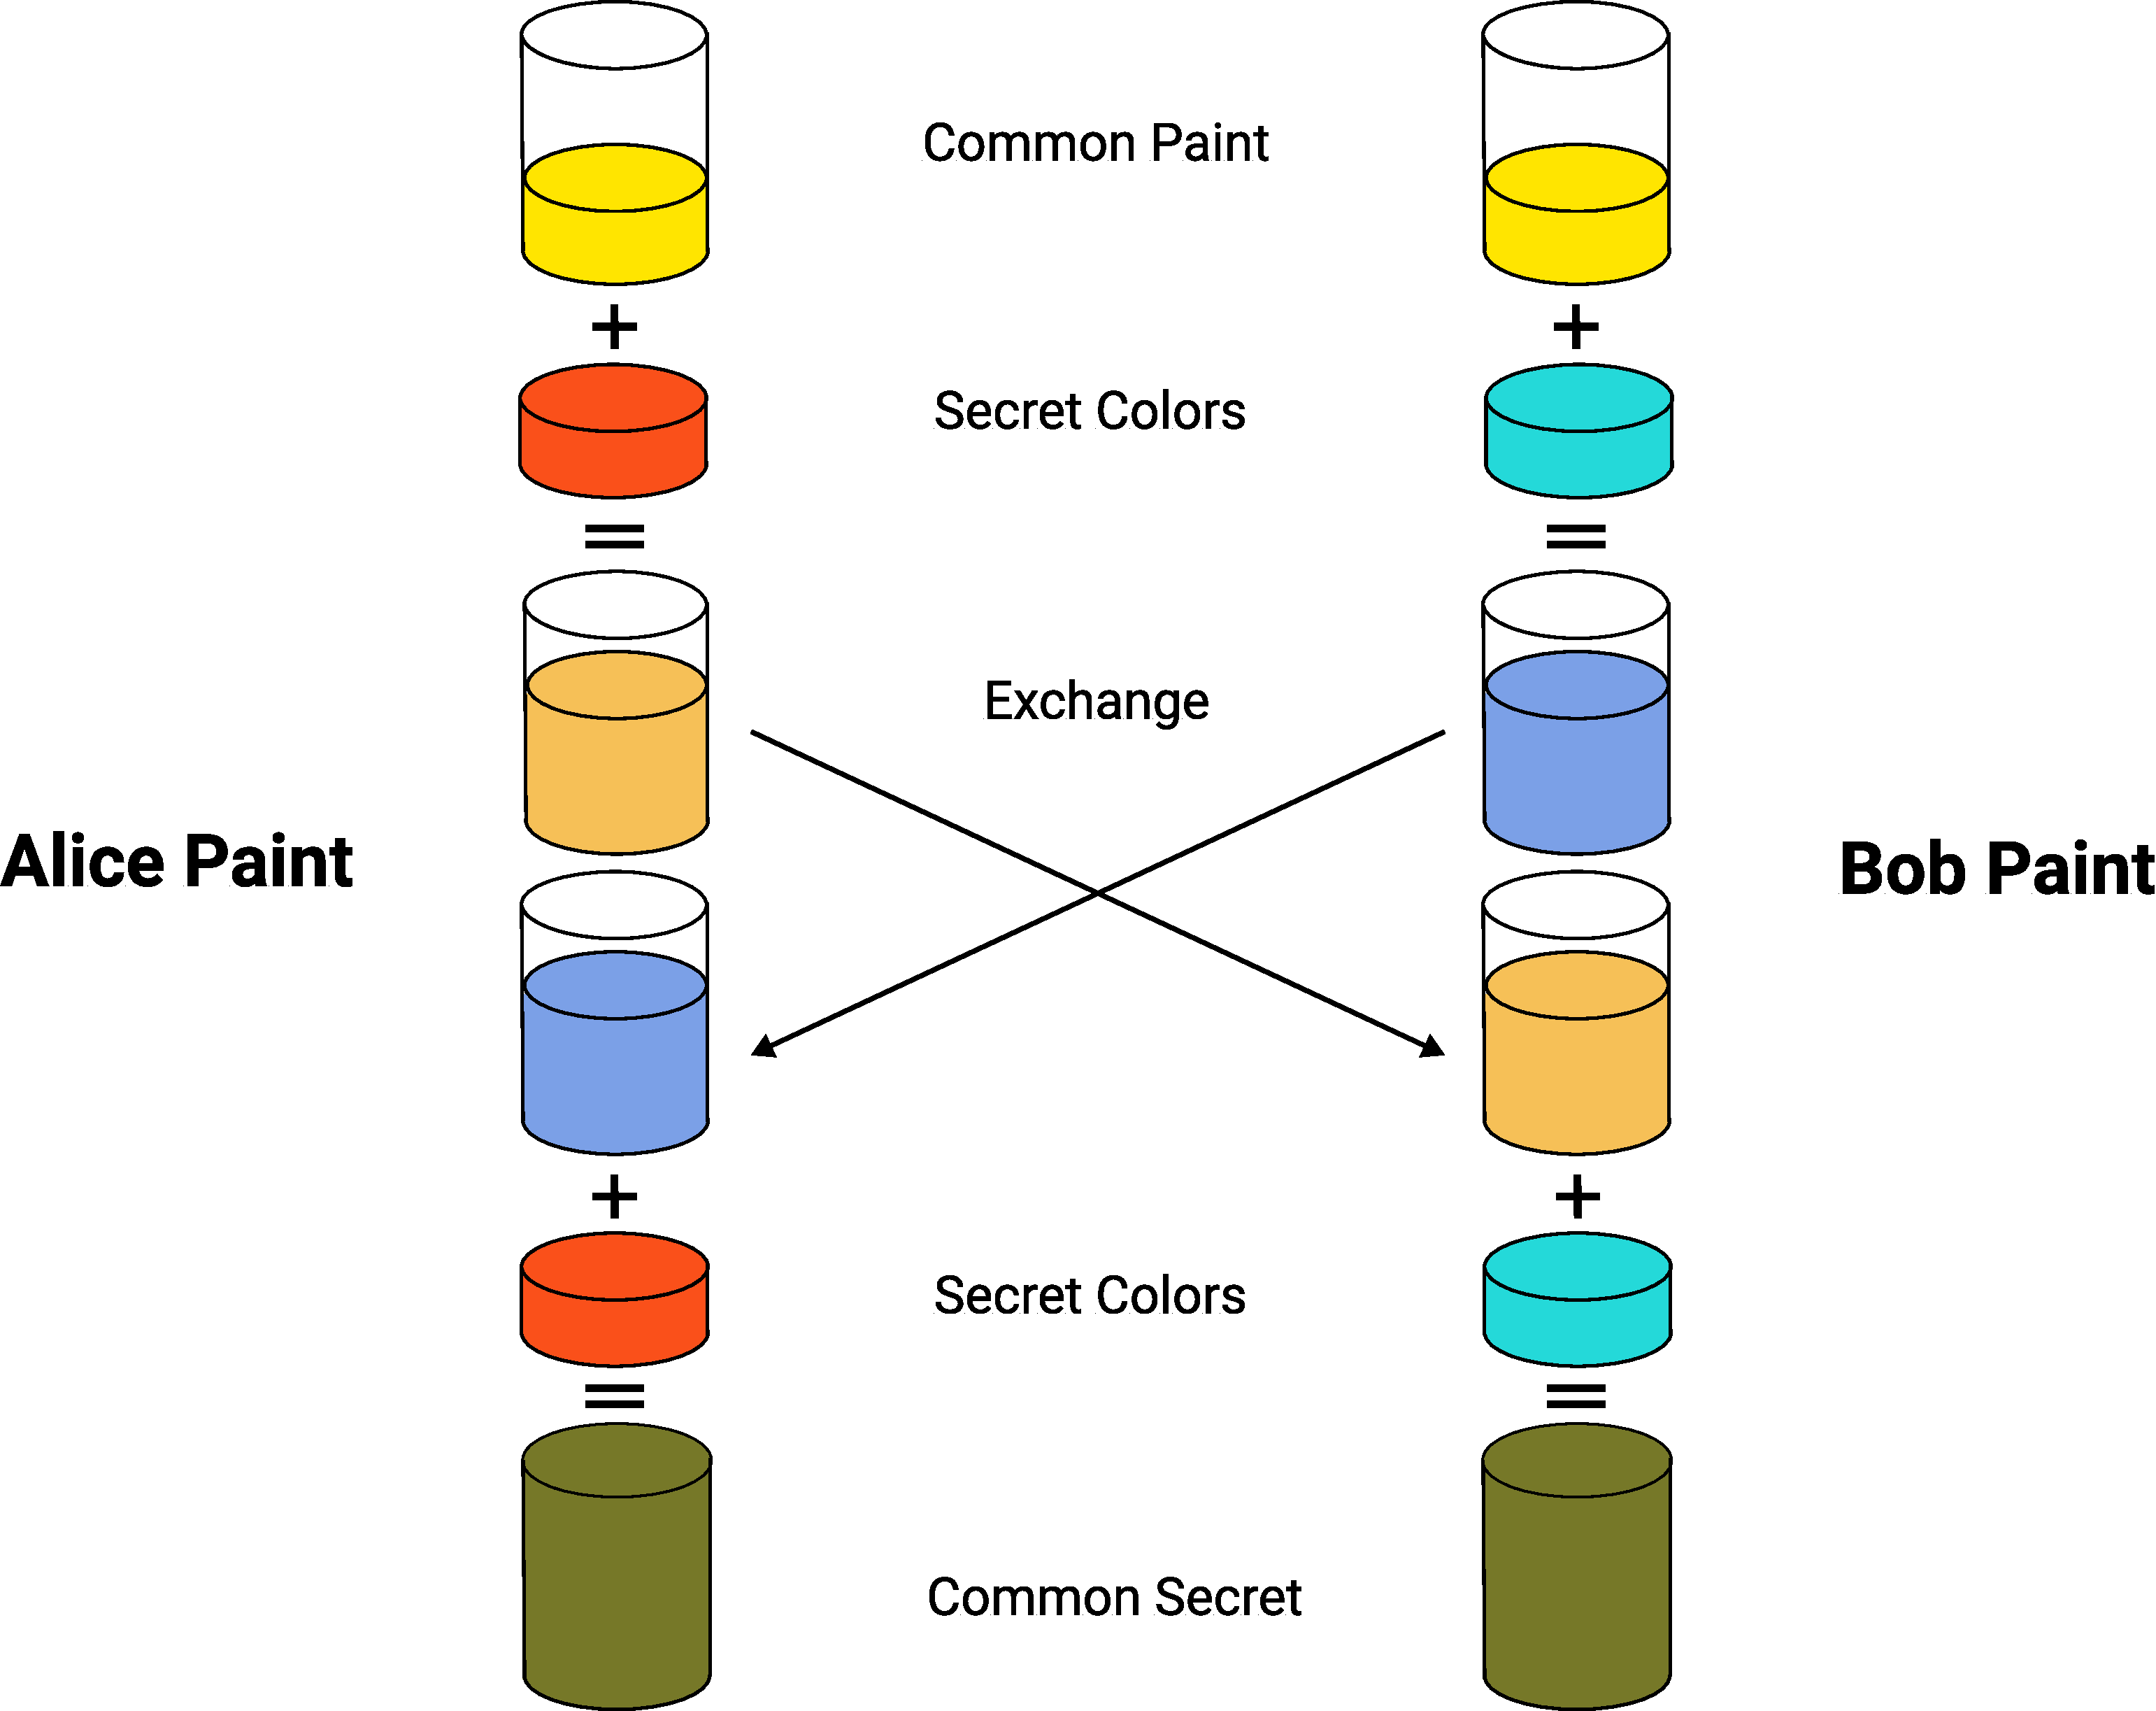
\includegraphics[width=1\textwidth]{Pictures/07_Diffie-Hellman_keyexchange_concept_diagram}
    \caption{Diffie–-Hellman key exchange concept diagram. Source: }\label{fig:figure4}
\end{figure}
In contrast to the Diffie–-Hellman based on discrete logarithm problem, there is an Elliptic Curve Diffie–-Hellman
key exchange, which based on the elliptic curve discrete logarithm problem.
Although, the idea is quite same, the difference only in that Elliptic Curve Diffie–-Hellman ensures the same safety
as discrete logarithm Diffie–-Hellman with lower value of the prime modulus $P$.
For instance, 521 bit modulus used in Elliptic Curve Diffie–-Hellman is equally safe as 2048 bit modulus in
discrete logarithm Diffie–-Hellman.
To summarize, the flow of Diffie–-Hellman key exchange is as follows
\begin{enumerate}
    \item Given 2048 bits prime modulus $P$ and generator $G$, such that $G$ is primitive root modulo $P$.
    \item Alice chooses her secret $a$.
    \item Alice sends to Bob her public key $A = G^a \bmod P$.
    \item Bob chooses his secret $b$.
    \item Bob sends to Alice his public key $B = G^b \bmod P$.
    \item Alice computes common secret $s = B^a \bmod P$.
    \item Bob computes common secret $s = A^b \bmod P$.
    \item Alice and Bob have arrived to the same value
    \begin{eqnarray}
        A^b \bmod P = G^{ab} \bmod P \\
        B^a \bmod P = G^{ba} \bmod P
    \end{eqnarray}
\end{enumerate}

\textbf{Implementation.} Although, the idea of DH key exchange looks quite simple, some remarks on the concrete
implementation should be added.
Firstly, it is necessary to implement the mechanism of key exchange request between two or more parties.
As it discussed above, each user has his own private-public keys pair, so in order to perform request between parties,
it should be implemented dedicate REST API endpoint, for instance the POST one \texttt{api/key-exchange-requests} which
takes the body of the form

\begin{spverbatim}
{
    "requestedUserId": "3fa85f64-5717-4562-b3fc-2c963f66afa6",
    "publicKey": "RUNLMSAAAAC2lkqYcTGhutQPxcjvoqUELKoy0"
}
\end{spverbatim}

So, request sender generates on the client side a key pair, keeps private on in the file system and shares the public
in request to receiver.
Therefore, the second party has received the key exchange request.
In order to display all the key exchange requests awaiting the confirmation of decline decisions, it is worth to implement
another REST endpoint such that GET \texttt{api/key-exchange-requests}, so that requested party will have the list of
requests to proceed.
This endpoint may return the data structure like follows

\begin{spverbatim}
{
    "keyExchangeRequests": [
        {
            "requestId": "81d314c1-913f-4686-827e-ef2a65ccc370",
            "senderId": "3fa85f64-5717-4562-b3fc-2c963f66afa6",
            "senderPublicKey": "RUNLMSAAAAC2lkqYcTGhutQPxcjvoqUELKoy0"
        }
    ],
    "message": "SUCCESS",
    "success": true
}
\end{spverbatim}

Finally, requested party should be able to confirm or decline the key exchange request, the DELETE endpoint
\texttt{api/key-exchange-requests} should be implemented then.
The server is able to fetch the request thanks to the body endpoint takes

\begin{spverbatim}
{
    "requestId": "3fa85f64-5717-4562-b3fc-2c963f66afa6",
    "confirmed": true,
    "publicKey": "string"
}
\end{spverbatim}

Therefore, an identifier of awaiting request is passed to the server among with boolean value
indicating the confirmation.
Under the roof of this operation are also generation of private-public keys pair for the requested party and
generation of common secret stored in client's file system.
As result, the initial request sender receives a public key as confirmation from requested party.
Requested side may get all his public keys via the REST API using GET \texttt{api/public-keys}

\begin{spverbatim}
{
    "publicKeys": [
        {
            "partnerId": "ae9e10a4-0c7e-4911-8450-4139d4a114a7",
            "partnerPublicKey": "RUNLMSAAAAAbc49wfaZ+QF9J2cu1S66bkp0"
        }
    ],
    "message": "SUCCESS",
    "success": true
}
\end{spverbatim}

Now requested participant is able to derive the common secret.
In order to provide an example, a simple command line interface is implemented.
We have used an Elliptic Curve Diffie–-Hellman implementation \texttt{ECDiffieHellmanCng Class} from the namespace
\texttt{System.Security.Cryptography} of the .NET base class library.
The \texttt{P-256} curve is used.

More precisely, the following CLI commands are implemented
\begin{itemize}
    \item \texttt{MangoAPI.DiffieHellmanConsole login SENDER\_EMAIL SENDER\_PASSWORD}
    \item \texttt{MangoAPI.DiffieHellmanConsole key-exchange RECEIVER\_ID}
    \item \texttt{MangoAPI.DiffieHellmanConsole key-exchange-requests}
    \item \texttt{MangoAPI.DiffieHellmanConsole confirm-key-exchange REQUEST\_ID}
    \item \texttt{MangoAPI.DiffieHellmanConsole print-public-keys}
    \item \texttt{MangoAPI.DiffieHellmanConsole create-common-secret RECEIVER\_ID}
\end{itemize}
Commands are self-explanatory, therefore we skip the detailed documentation on them.
An example of console output straightforward
\begin{figure}[H]
    \centering
    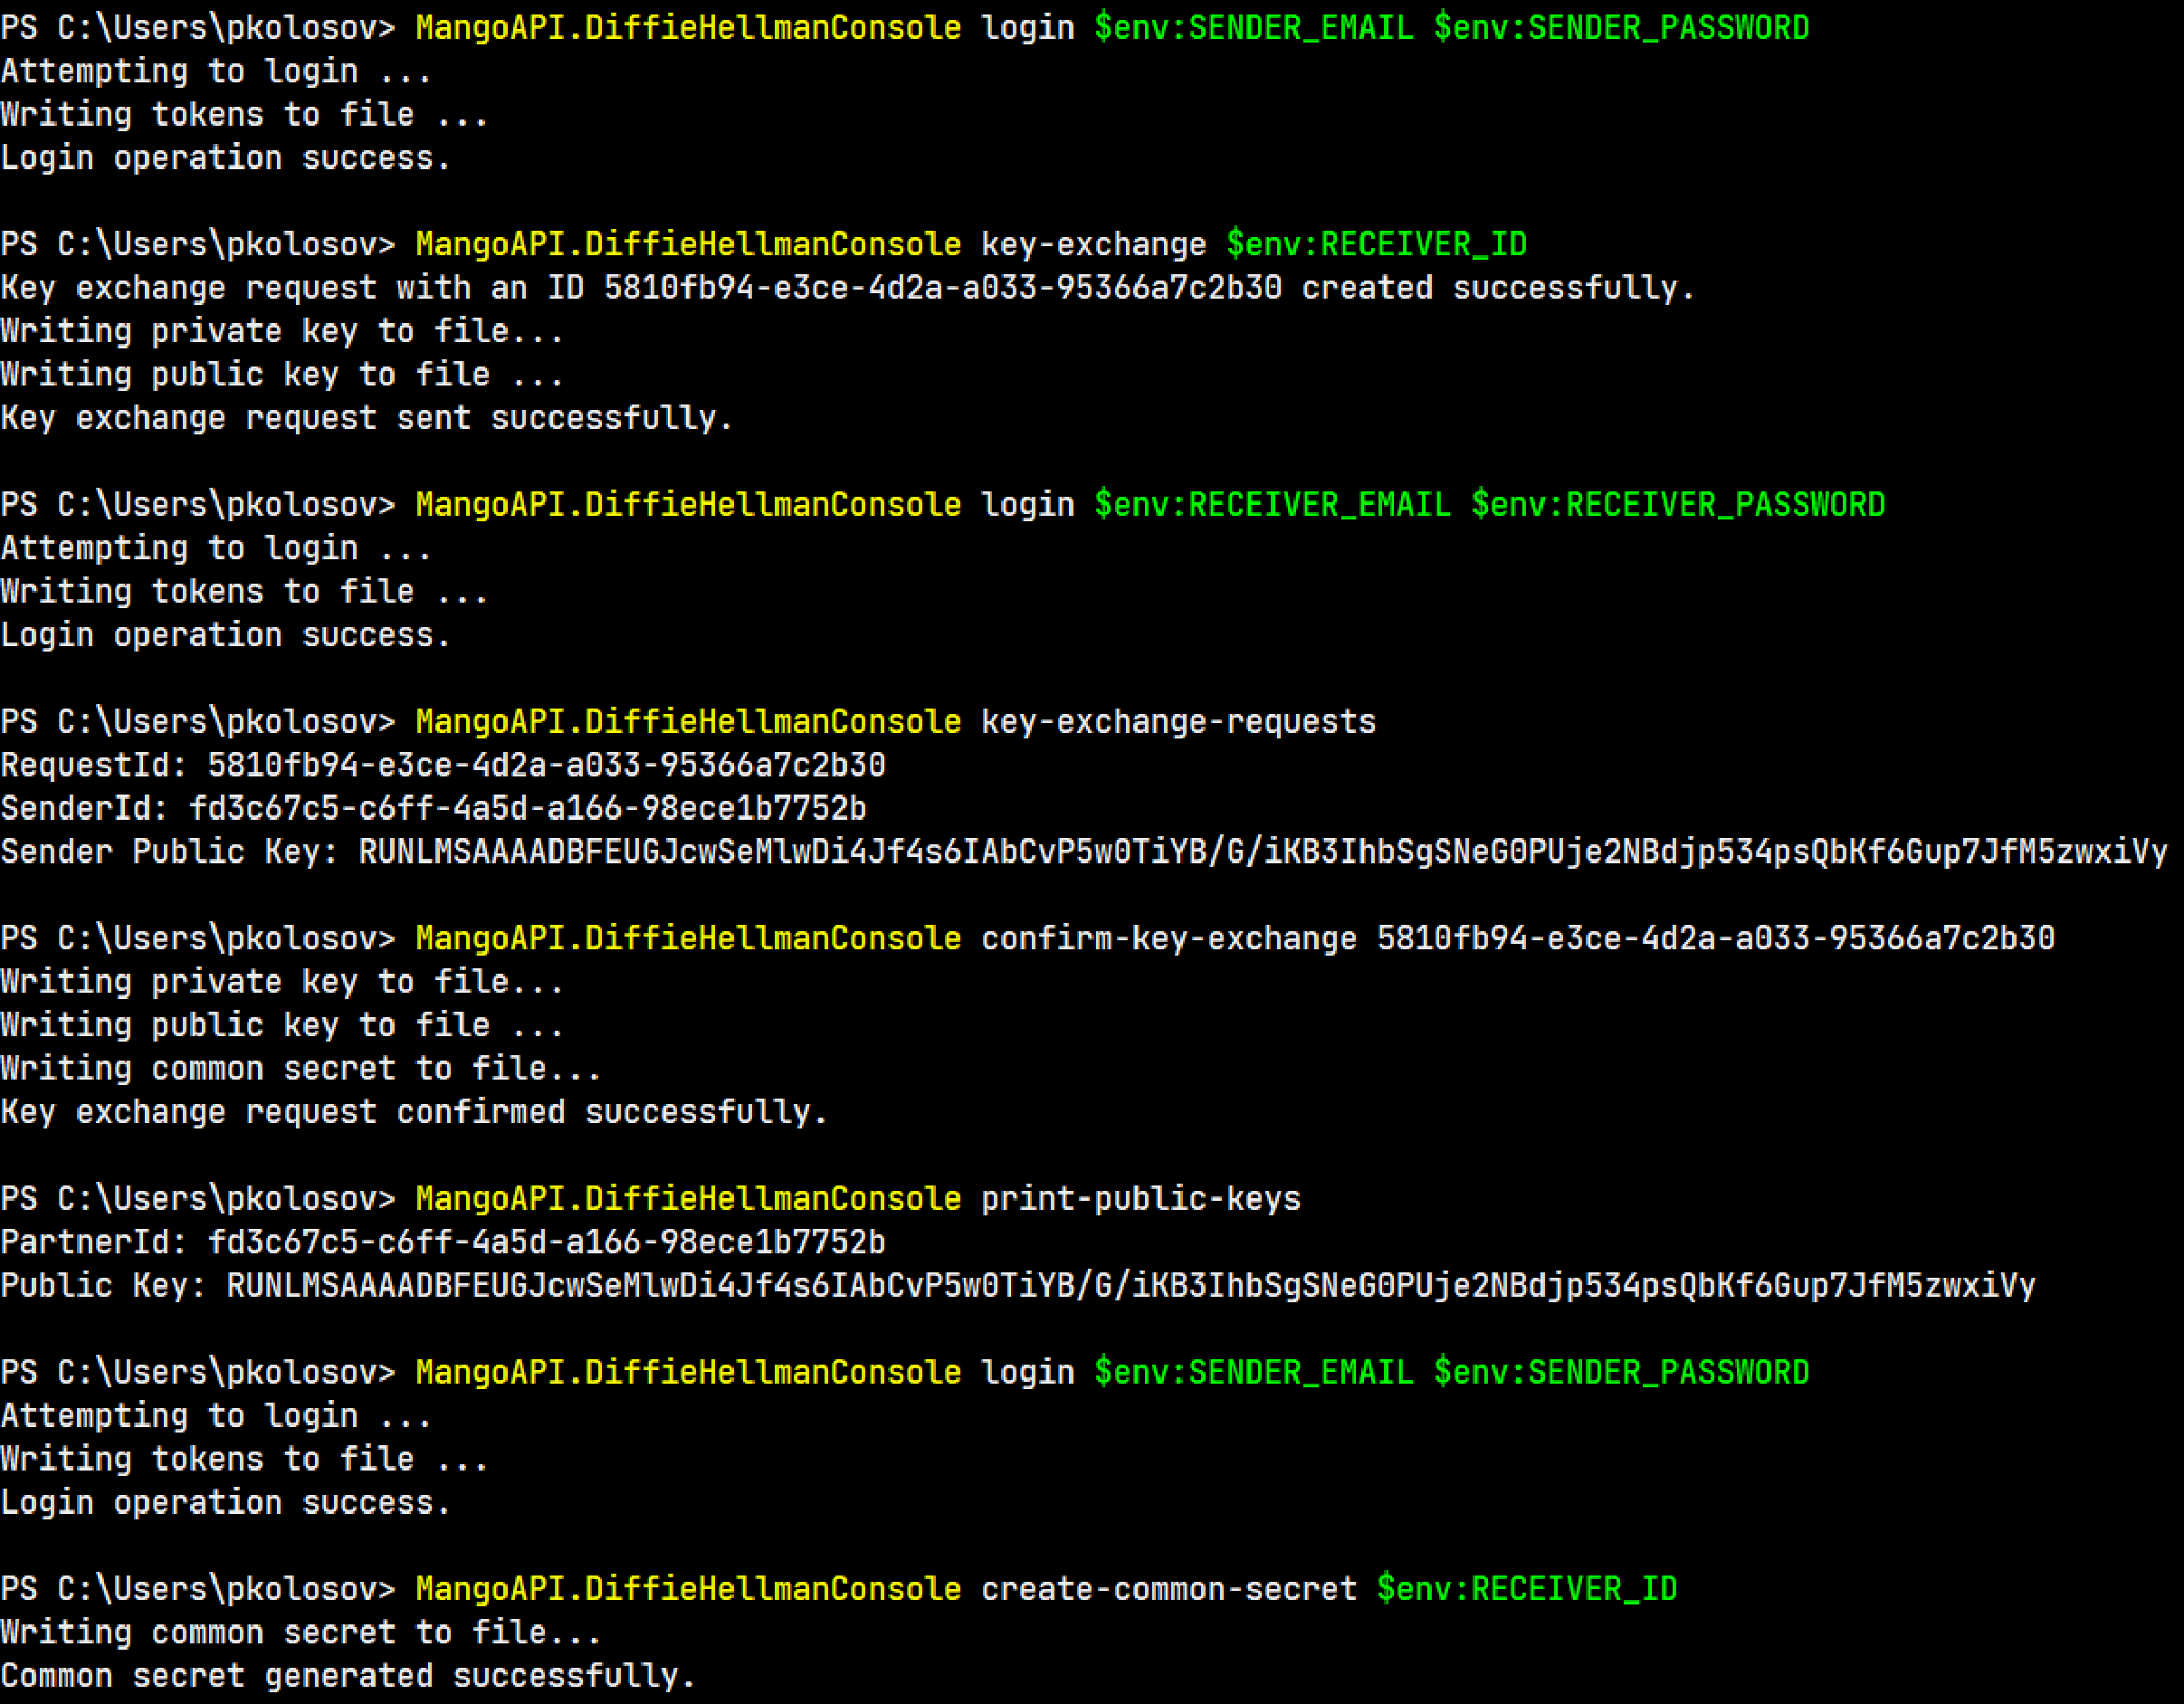
\includegraphics[width=1\textwidth]{Pictures/08_Diffie-Hellman_console_output}
    \caption{Diffie–-Hellman key exchange console output. Source: }\label{fig:figure7}
\end{figure}
Finally, both test accounts reached the same common secret.